\documentclass[uplatex,dvipdfmx]{jsarticle}
\title{記号論理学レポート(担当:岡本賢吾先生)}
\author{司馬博文 J4-190549}
\pagestyle{plain}
\usepackage{amsmath, amsfonts, amsthm, amssymb, ascmac, color, comment, wrap fig}

\setcounter{tocdepth}{2}
%2はsubsectionまで
\usepackage{mathtools}
%\mathtoolsset{showonlyrefs=true} %labelを附した数式にのみ附番される.

%%% 生成されるPDFファイルにおいて、\tableofcontents によって書き出された目次をクリックすると該当する見出しへジャンプしたり、 さらには、\label{ラベル名} を番号で参照する \ref{ラベル名} や thebibliography環境において \bibitem{ラベル名} を文献番号で参照する \cite{ラベル名} においても番号をクリックすると該当箇所にジャンプする
\usepackage[dvipdfmx]{hyperref}
\usepackage{pxjahyper}

\usepackage{tikz, tikz-cd}
\usepackage[all]{xy}
\def\objectstyle{\displaystyle} %デフォルトではxymatrix中の数式が文中数式モードになるので,それを直した.

%化学式をTikZで簡単に書くためのパッケージ.
\usepackage[version=4]{mhchem} %texdoc mhchem
%化学構造式をTikZで描くためのパッケージ.
\usepackage{chemfig}
%IS単位を書くためのパッケージ
\usepackage{siunitx}

%取り消し線を引くためのパッケージ
\usepackage{ulem}

%\rotateboxコマンドを,文字列の中心で回転させるオプション.
%他rotatebox, scalebox, reflectbox, resizeboxなどのコマンド.
\usepackage{graphicx}

%加藤晃史さんがフル活用していたtcolorboxを,途中改ページ可能で.
\usepackage[breakable]{tcolorbox}

%足助さんからもらったオプション
% \usepackage[shortlabels,inline]{enumitem}
% \usepackage[top=15truemm,bottom=15truemm,left=10truemm,right=10truemm]{geometry}

%enumerate環境を凝らせる.
\usepackage{enumerate}

%日本語にルビをふる
\usepackage{pxrubrica}

%以下,ソースコードを表示する環境の設定.
\usepackage{listings,jvlisting} %日本語のコメントアウトをする場合jlistingが必要
%ここからソースコードの表示に関する設定
\lstset{
  basicstyle={\ttfamily},
  identifierstyle={\small},
  commentstyle={\smallitshape},
  keywordstyle={\small\bfseries},
  ndkeywordstyle={\small},
  stringstyle={\small\ttfamily},
  frame={tb},
  breaklines=true,
  columns=[l]{fullflexible},
  numbers=left,
  xrightmargin=0zw,
  xleftmargin=3zw,
  numberstyle={\scriptsize},
  stepnumber=1,
  numbersep=1zw,
  lineskip=-0.5ex
}
%lstlisting環境で,[caption=hoge,label=fuga]などのoptionを付けられる.

%%%
%%%フォント
%%%

%本文・数式の両方のフォントをTimesに変更するお手軽なパッケージだが,LaTeX標準数式記号の\jmath, \amalg, coprodはサポートされない.
\usepackage{mathptmx}
%Palatinoの方が完成度が高いと美文書作成に書いてあった.
% \usepackage[sc]{mathpazo} %オプションは,familyの指定.pplxにしている.
%2000年のYoung Ryuによる新しいTimes系.なおPalatinoもある.
% \usepackage{newtxtext, newtxmath}
%拡張数学記号.\textsectionでブルバキに!
% \usepackage{textcomp, mathcomp}
% \usepackage[T1]{fontenc} %8bitエンコーディングにする.comp系拡張数学文字の動作が安定する.
%AMS Euler.Computer Modernと相性が悪いとは…….
% \usepackage{ccfonts, eulervm} %KnuthのConcrete Mathematicsの組み合わせ.
% \renewcommand{\rmdefault}{pplx} %makes LaTeX use Palatino in place of CM Roman.Do not use the Euler math fonts in conjunction with the default Computer Modern text fonts – this is ugly!

%%% newcommands
    %参考文献で⑦というのを出したかった.\circled{n}と打てば良い.LaTeX StackExchangeより.
\newcommand*\circled[1]{\tikz[baseline=(char.base)]{\node[shape=circle,draw,inner sep=0.8pt] (char) {#1};}}

%%%
%%% ショートカット 足助さんからのコピペ
%%%

\DeclareMathOperator{\grad}{\mathrm{grad}}
\DeclareMathOperator{\rot}{\mathrm{rot}}
\DeclareMathOperator{\divergence}{\mathrm{div}}
\newcommand\R{\mathbb{R}}
\newcommand\N{\mathbb{N}}
\newcommand\C{\mathbb{C}}
\newcommand\Z{\mathbb{Z}}
\newcommand\Q{\mathbb{Q}}
\newcommand\GL{\mathrm{GL}}
\newcommand\SL{\mathrm{SL}}
\newcommand\False{\mathrm{False}}
\newcommand\True{\mathrm{True}}
\newcommand\tr{\mathrm{tr}}
\newcommand\M{\mathcal{M}}
\newcommand\F{\mathbb{F}}
\renewcommand\H{\mathbb{H}}
\newcommand\id{\mathrm{id}}
\newcommand\A{\mathcal{A}}
\renewcommand\coprod{\rotatebox[origin=c]{180}{$\prod$}}
\newcommand\pr{\mathrm{pr}}
\newcommand\U{\mathfrak{U}}
\newcommand\Map{\mathrm{Map}}
\newcommand\dom{\mathrm{dom}}
\newcommand\cod{\mathrm{cod}}
\newcommand\supp{\mathrm{supp}\;}
\newcommand\Ker{\mathrm{Ker}\;}
%%% 複素解析学
\renewcommand\Re{\mathrm{Re}\;}
\renewcommand\Im{\mathrm{Im}\;}
\newcommand\Gal{\mathrm{Gal}}
\newcommand\PGL{\mathrm{PGL}}
\newcommand\PSL{\mathrm{PSL}}
%%% 解析力学
\newcommand\x{\mathbf{x}}
\newcommand\q{\mathbf{q}}
%%% 集合と位相
\newcommand\ORD{\mathrm{ORD}}
%%% 形式言語理論
\newcommand\REGEX{\mathrm{REGEX}}

%%% 圏
\newcommand\Hom{\mathrm{Hom}}
\newcommand\Mor{\mathrm{Mor}}
\newcommand\Aut{\mathrm{Aut}}
\newcommand\End{\mathrm{End}}
\newcommand\op{\mathrm{op}}
\newcommand\ev{\mathrm{ev}}
\newcommand\Ob{\mathrm{Ob}}
\newcommand\Ar{\mathrm{Ar}}
\newcommand\Arr{\mathrm{Arr}}
\newcommand\Set{\mathrm{Set}}
\newcommand\Grp{\mathrm{Grp}}
\newcommand\Cat{\mathrm{Cat}}
\newcommand\Mon{\mathrm{Mon}}
\newcommand\CMon{\mathrm{CMon}}
\newcommand\Pos{\mathrm{Pos}}
\newcommand\Vect{\mathrm{Vect}}
\newcommand\FinVect{\mathrm{FinVect}}
\newcommand\Fun{\mathrm{Fun}}
\newcommand\Ord{\mathrm{Ord}}
\newcommand\eq{\mathrm{eq}}
\newcommand\coeq{\mathrm{coeq}}

%%%
%%% 定理環境 以下足助さんからのコピペ
%%%

\newtheoremstyle{StatementsWithStar}% ?name?
{3pt}% ?Space above? 1
{3pt}% ?Space below? 1
{}% ?Body font?
{}% ?Indent amount? 2
{\bfseries}% ?Theorem head font?
{\textbf{.}}% ?Punctuation after theorem head?
{.5em}% ?Space after theorem head? 3
{\textbf{\textup{#1~\thetheorem{}}}{}\,$^{\ast}$\thmnote{(#3)}}% ?Theorem head spec (can be left empty, meaning ‘normal’)?
%
\newtheoremstyle{StatementsWithStar2}% ?name?
{3pt}% ?Space above? 1
{3pt}% ?Space below? 1
{}% ?Body font?
{}% ?Indent amount? 2
{\bfseries}% ?Theorem head font?
{\textbf{.}}% ?Punctuation after theorem head?
{.5em}% ?Space after theorem head? 3
{\textbf{\textup{#1~\thetheorem{}}}{}\,$^{\ast\ast}$\thmnote{(#3)}}% ?Theorem head spec (can be left empty, meaning ‘normal’)?
%
\newtheoremstyle{StatementsWithStar3}% ?name?
{3pt}% ?Space above? 1
{3pt}% ?Space below? 1
{}% ?Body font?
{}% ?Indent amount? 2
{\bfseries}% ?Theorem head font?
{\textbf{.}}% ?Punctuation after theorem head?
{.5em}% ?Space after theorem head? 3
{\textbf{\textup{#1~\thetheorem{}}}{}\,$^{\ast\ast\ast}$\thmnote{(#3)}}% ?Theorem head spec (can be left empty, meaning ‘normal’)?
%
\newtheoremstyle{StatementsWithCCirc}% ?name?
{6pt}% ?Space above? 1
{6pt}% ?Space below? 1
{}% ?Body font?
{}% ?Indent amount? 2
{\bfseries}% ?Theorem head font?
{\textbf{.}}% ?Punctuation after theorem head?
{.5em}% ?Space after theorem head? 3
{\textbf{\textup{#1~\thetheorem{}}}{}\,$^{\circledcirc}$\thmnote{(#3)}}% ?Theorem head spec (can be left empty, meaning ‘normal’)?
%
\theoremstyle{definition}
 \newtheorem{theorem}{定理}[section]
 \newtheorem{axiom}[theorem]{公理}
 \newtheorem{corollary}[theorem]{系}
 \newtheorem{proposition}[theorem]{命題}
 \newtheorem*{proposition*}{命題}
 \newtheorem{lemma}[theorem]{補題}
 \newtheorem*{lemma*}{補題}
 \newtheorem*{theorem*}{定理}
 \newtheorem{definition}[theorem]{定義}
 \newtheorem{example}[theorem]{例}
 \newtheorem{notation}[theorem]{記法}
 \newtheorem*{notation*}{記法}
 \newtheorem{assumption}[theorem]{仮定}
 \newtheorem{question}[theorem]{問}
 \newtheorem{counterexample}[theorem]{反例}
 \newtheorem{reidai}[theorem]{例題}
 \newtheorem{problem}[theorem]{問題}
 \newtheorem*{solution*}{\bf{[解]}}
 \newtheorem{discussion}[theorem]{議論}
 \newtheorem{remark}[theorem]{注}
 \newtheorem{universality}[theorem]{普遍性} %非自明な例外がない.
 \newtheorem{universal tendency}[theorem]{普遍傾向} %例外が有意に少ない.
 \newtheorem{hypothesis}[theorem]{仮説} %実験で説明されていない理論.
 \newtheorem{theory}[theorem]{理論} %実験事実とその(さしあたり)整合的な説明.
 \newtheorem{fact}[theorem]{実験事実}
 \newtheorem{model}[theorem]{模型}
 \newtheorem{explanation}[theorem]{説明} %理論による実験事実の説明
 \newtheorem{anomaly}[theorem]{理論の限界}
 \newtheorem{application}[theorem]{応用例}
 \newtheorem{method}[theorem]{手法} %実験手法など,技術的問題.
 \newtheorem{history}[theorem]{歴史}
 \newtheorem{research}[theorem]{研究}
% \newtheorem*{remarknonum}{注}
 \newtheorem*{definition*}{定義}
 \newtheorem*{remark*}{注}
 \newtheorem*{question*}{問}
 \newtheorem*{axiom*}{公理}
 \newtheorem*{example*}{例}
%
\theoremstyle{StatementsWithStar}
 \newtheorem{definition_*}[theorem]{定義}
 \newtheorem{question_*}[theorem]{問}
 \newtheorem{example_*}[theorem]{例}
 \newtheorem{theorem_*}[theorem]{定理}
 \newtheorem{remark_*}[theorem]{注}
%
\theoremstyle{StatementsWithStar2}
 \newtheorem{definition_**}[theorem]{定義}
 \newtheorem{theorem_**}[theorem]{定理}
 \newtheorem{question_**}[theorem]{問}
 \newtheorem{remark_**}[theorem]{注}
%
\theoremstyle{StatementsWithStar3}
 \newtheorem{remark_***}[theorem]{注}
 \newtheorem{question_***}[theorem]{問}
%
\theoremstyle{StatementsWithCCirc}
 \newtheorem{definition_O}[theorem]{定義}
 \newtheorem{question_O}[theorem]{問}
 \newtheorem{example_O}[theorem]{例}
 \newtheorem{remark_O}[theorem]{注}
%
\theoremstyle{definition}
%
\raggedbottom
\allowdisplaybreaks

%証明環境のスタイル
\everymath{\displaystyle}
\renewcommand{\proofname}{\bf [証明]}
\renewcommand{\thefootnote}{\dag\arabic{footnote}}	%足助さんからもらった.どうなるんだ?

%mathptmxパッケージ下で,\jmath, \amalg, coprodの記号を出力するためのマクロ.TeX Wikiからのコピペ.
% \DeclareSymbolFont{cmletters}{OML}{cmm}{m}{it}
% \DeclareSymbolFont{cmsymbols}{OMS}{cmsy}{m}{n}
% \DeclareSymbolFont{cmlargesymbols}{OMX}{cmex}{m}{n}
% \DeclareMathSymbol{\myjmath}{\mathord}{cmletters}{"7C}
% \DeclareMathSymbol{\myamalg}{\mathbin}{cmsymbols}{"71}
% \DeclareMathSymbol{\mycoprod}{\mathop}{cmlargesymbols}{"60}
% \let\jmath\myjmath
% \let\amalg\myamalg
% \let\coprod\mycoprod
\renewcommand\thesection{[\arabic{section}]}
\begin{document}
\maketitle
\begin{abstract}
    このレポートは,提示された問題[1]$\sim$[5]の問題文と解答からなる.また,記法上の注意や補題については各節の初めにまとめた.
    問題[5]では,筆者の興味の中心である自動定理証明システムとその数学の応用に関連して,Herbrandの定理の
    ステートメントの意味とその証明を自分の言葉で述べた.最後に問題[5]の解答の内容の執筆にあたって参考にした文献をまとめて附した.
\end{abstract}

\section{}

まず,問題を解く前にいくつか補題を示す.

\begin{lemma}
    \[\psi\vdash_{NJ,NK}\phi\to\psi\]
\end{lemma}
\begin{proof}\mbox{}\\
    \begin{center}
        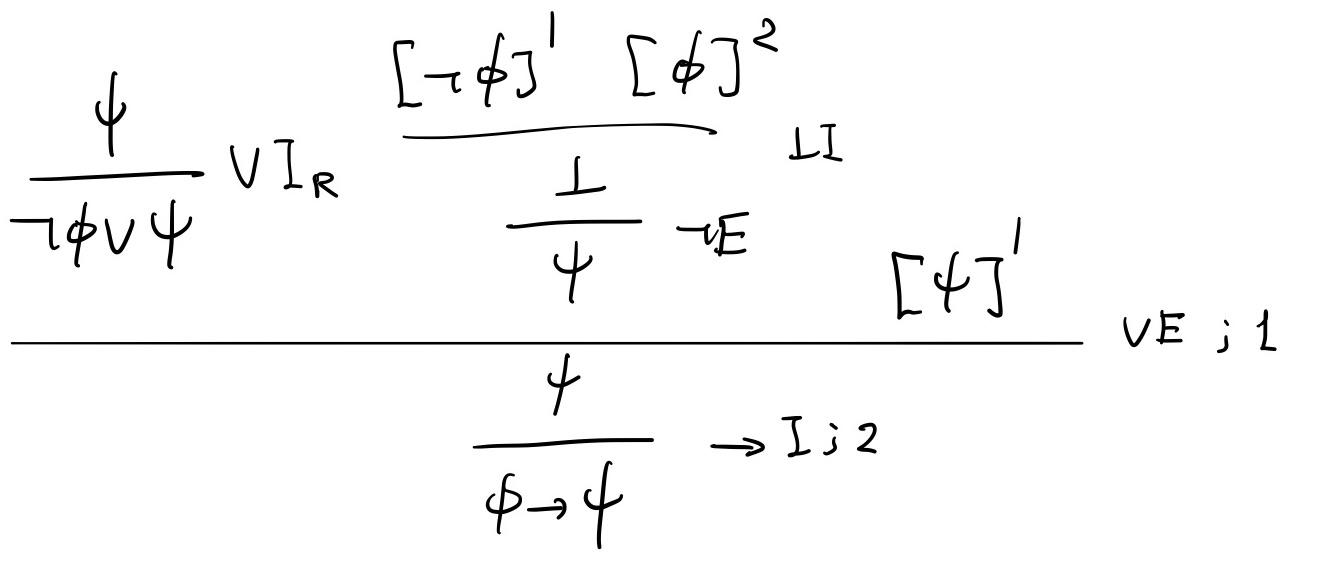
\includegraphics[width=15cm]{figure1.jpg}
    \end{center}
\end{proof}

\begin{lemma}[De Morgan's law]
    \[ \lnot(\phi\land\psi)\vdash_{NK}\lnot\phi\lor\lnot\psi \]
\end{lemma}
\begin{proof}
    次が証明図である.
    \begin{center}
        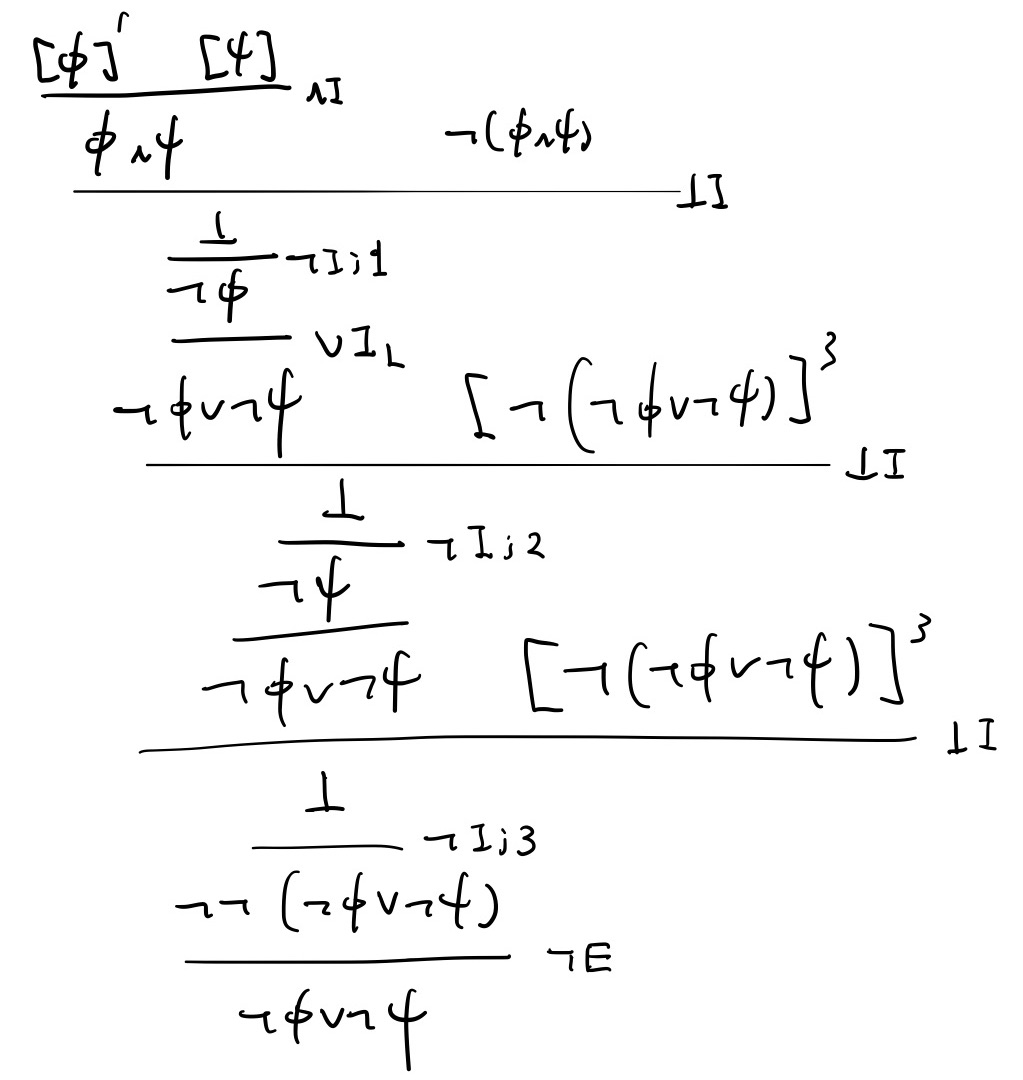
\includegraphics[width=15cm]{figure4.jpg}
    \end{center}
\end{proof}

これらの証明図は問題を解くにあたって参照される.

\begin{problem}[2007年度版(1)]
    \[\phi\to\lnot\phi,\lnot\lnot\psi\to\lnot\psi\vdash\lnot(\phi\lor\psi)\]
\end{problem}
\begin{proof}[\bf{[解]}]この証明図は次の通り.
    \begin{center}
        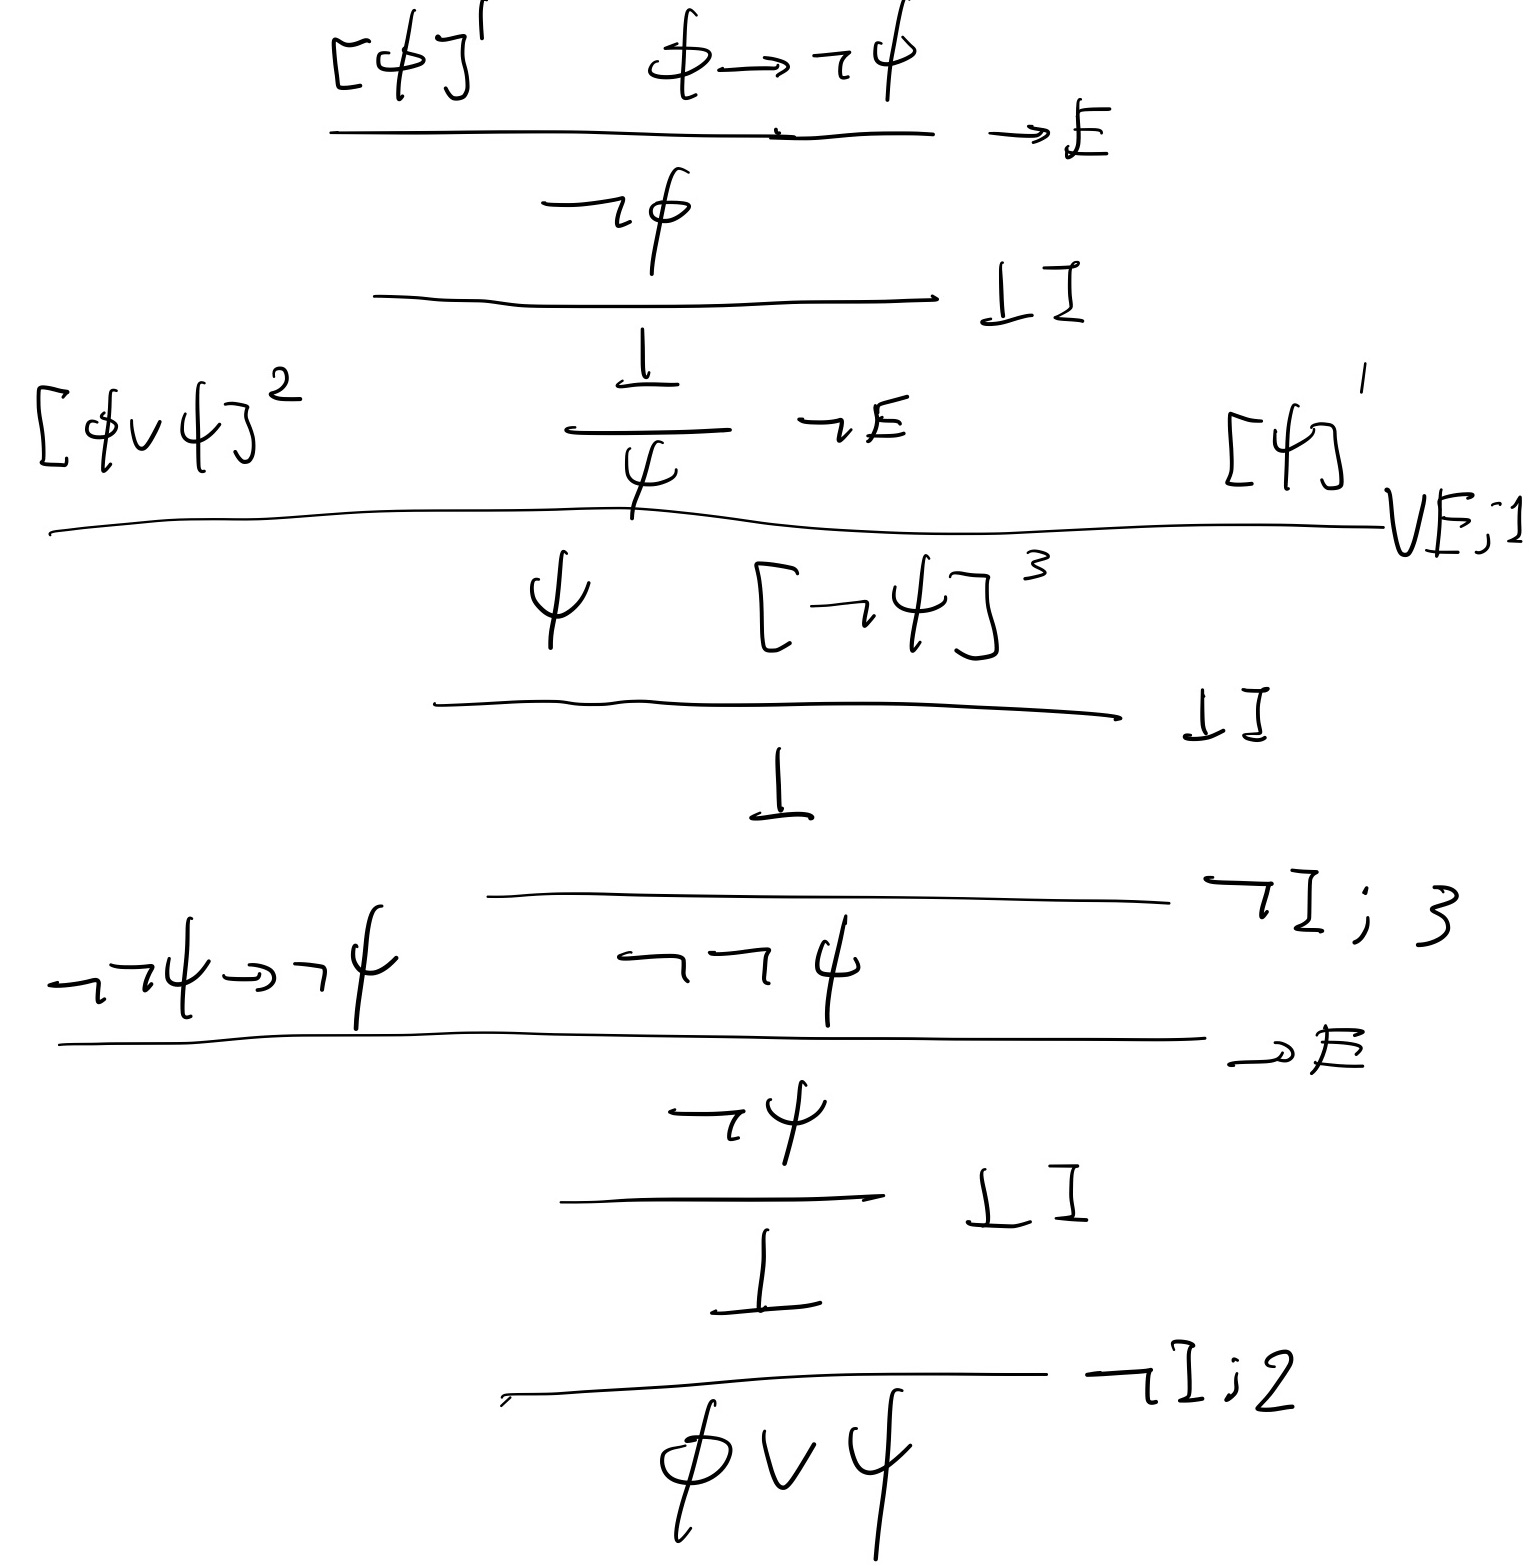
\includegraphics[width=15cm]{figure2.jpg}
    \end{center}
\end{proof}

\begin{problem}[2007年度版(2)]
    \[(\phi\to\psi)\to(X\lor(\psi\to\phi)),X\to(\phi\lor\lnot\psi)\vdash\psi\to\phi\]
\end{problem}
\begin{proof}[\bf{[解]}]この証明図は次の通り.
    \begin{center}
        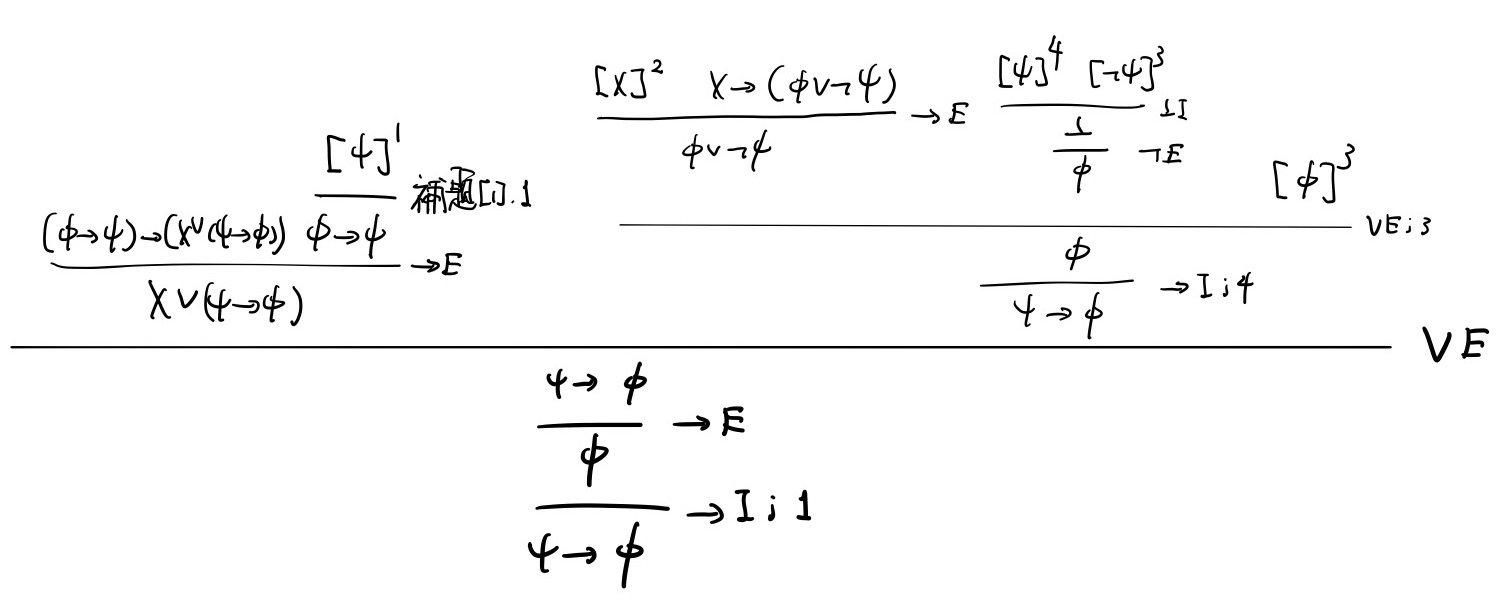
\includegraphics[width=15cm]{figure3.jpg}
    \end{center}
\end{proof}

\begin{problem}[2007年度版(3)]
    \[\phi\to\forall(\psi(x)\lor\Omega)\vdash_{NK}(\phi\to\forall x\psi(x))\lor\Omega\]
\end{problem}
\begin{proof}[\bf{[解]}]
    次が証明図である.ただし,$t$は仮定$\Phi$には自由出現しない任意な変数とした.
    \begin{center}
        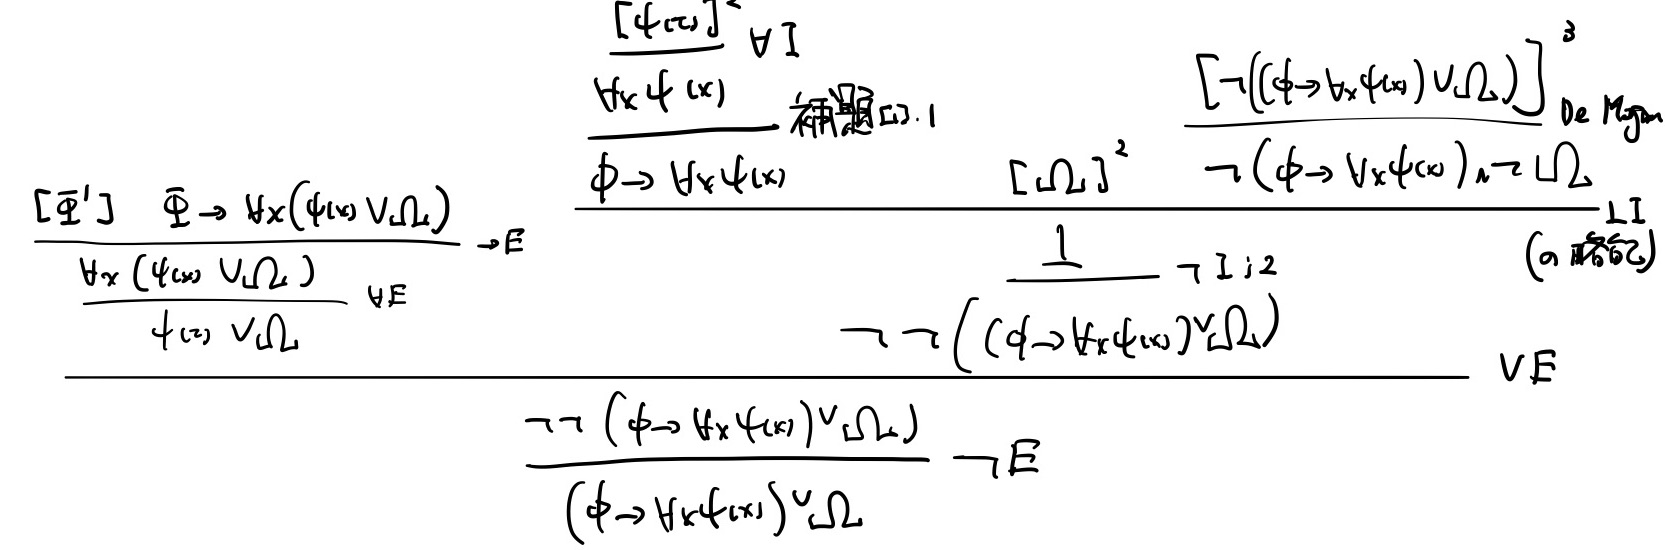
\includegraphics[width=15cm]{figure5.jpg}
    \end{center}
\end{proof}

\begin{problem}[2008年度版(1)]
    \[\phi\to(\lnot\phi\lor\psi)\vdash\phi\to\lnot(\psi\to(\lnot\phi\lor\lnot\psi))\]
\end{problem}
\begin{proof}[\bf{[解]}]
    証明図は次の通りである.
    \begin{center}
        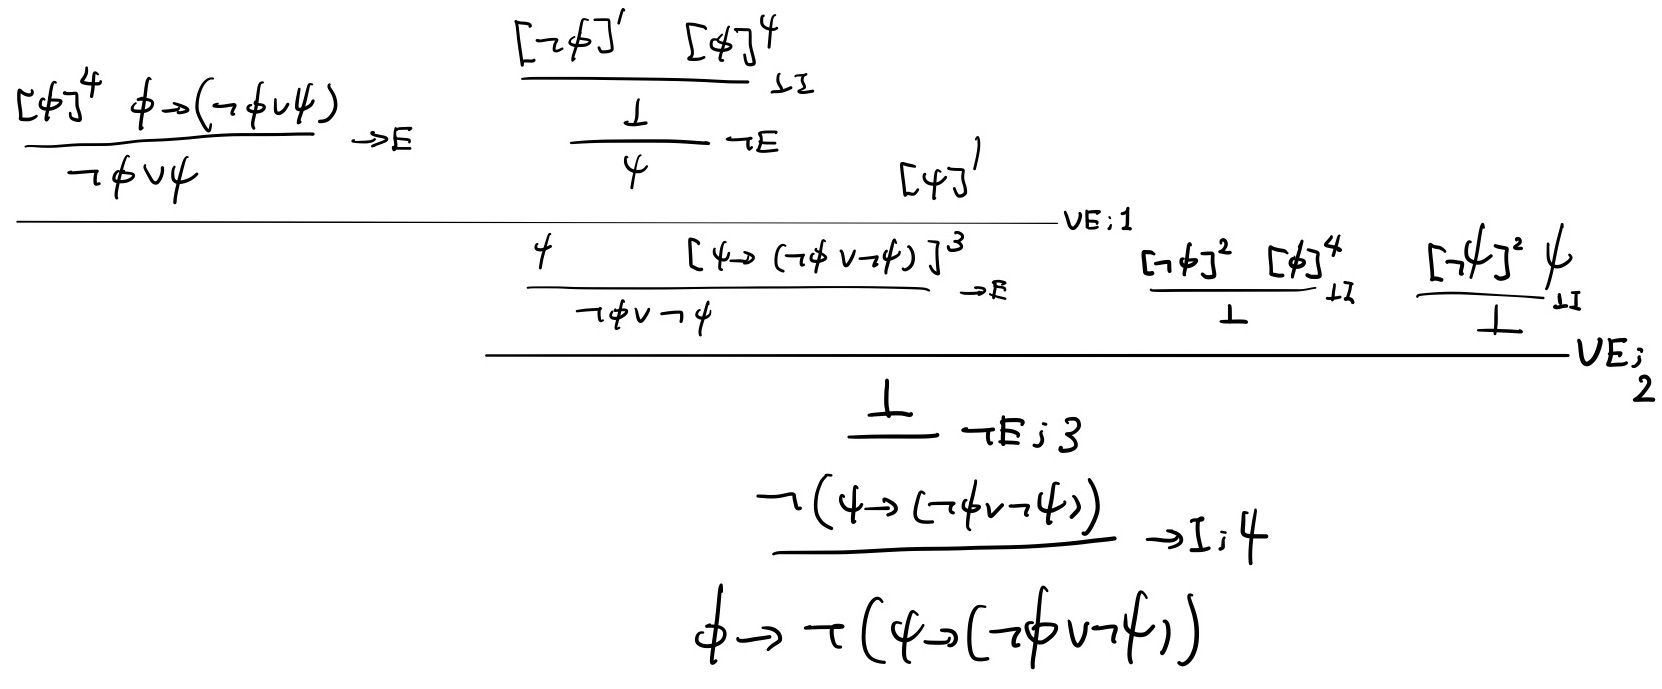
\includegraphics[width=15cm]{figure6.jpg}
    \end{center}
\end{proof}

\section{}

まず1つ補題を用意する.

\begin{lemma}[De Morgan's law]
    \[ \lnot(\Phi\lor\Psi)\vdash\lnot\Phi\land\lnot\Psi \]
\end{lemma}
\begin{proof}
    次が証明図である.
    \begin{center}
        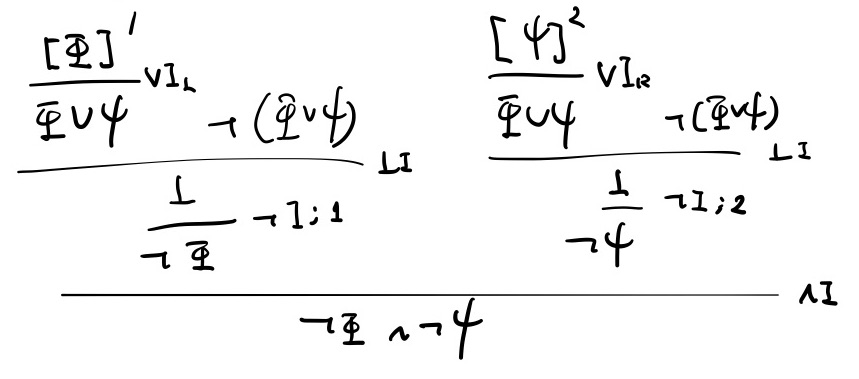
\includegraphics[width=15cm]{figure_demorgan.jpg}
    \end{center}
\end{proof}

以降,記号(1)$\sim$(10),[A]$\sim$[D]は問題文内で定義された命題(の集合)を表すものとする.
\begin{problem}
    \[ (1),(2),(3),(4),(5),(6),(7),(8),(9),(10)\vdash\bot\;\;\;\;\;\cdots[*] \]
\end{problem}
\begin{proof}[\bf{[解]}]
    まず,5つの部分証明図を用意する.
    部分証明図$\frac{(1)\;\;\;\;(2)}{[A]\lor[B]\lor[C]\lor[D]}\;\Pi_1$は次の通りである.
    \begin{center}
        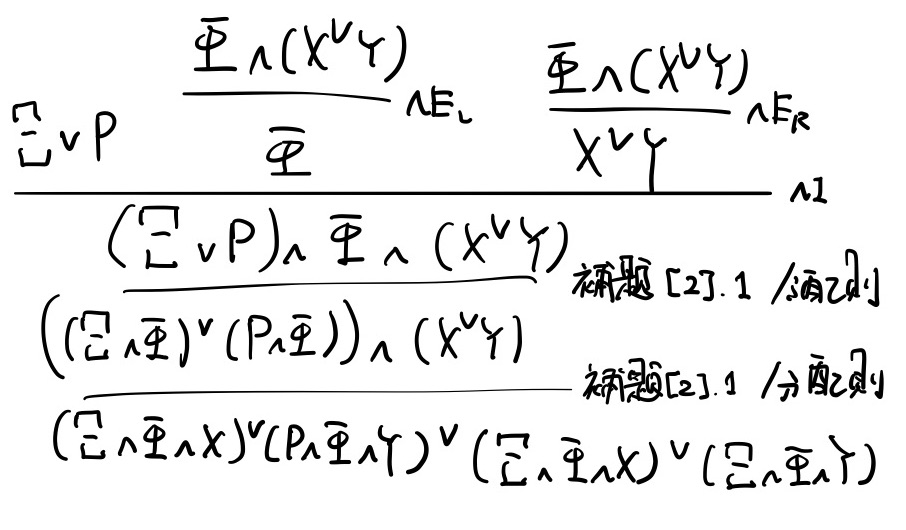
\includegraphics[width=15cm]{figure7.jpg}
    \end{center}
    部分証明図$\frac{[A]}{\bot}\Pi_2$は次の通りである.
    \begin{center}
        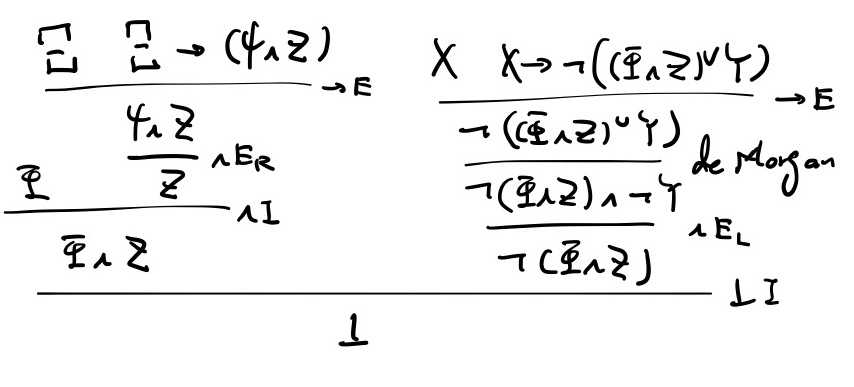
\includegraphics[width=15cm]{figure8.jpg}
    \end{center}
    部分証明図$\frac{[B]}{\bot}\Pi_3$は次の通りである.
    \begin{center}
        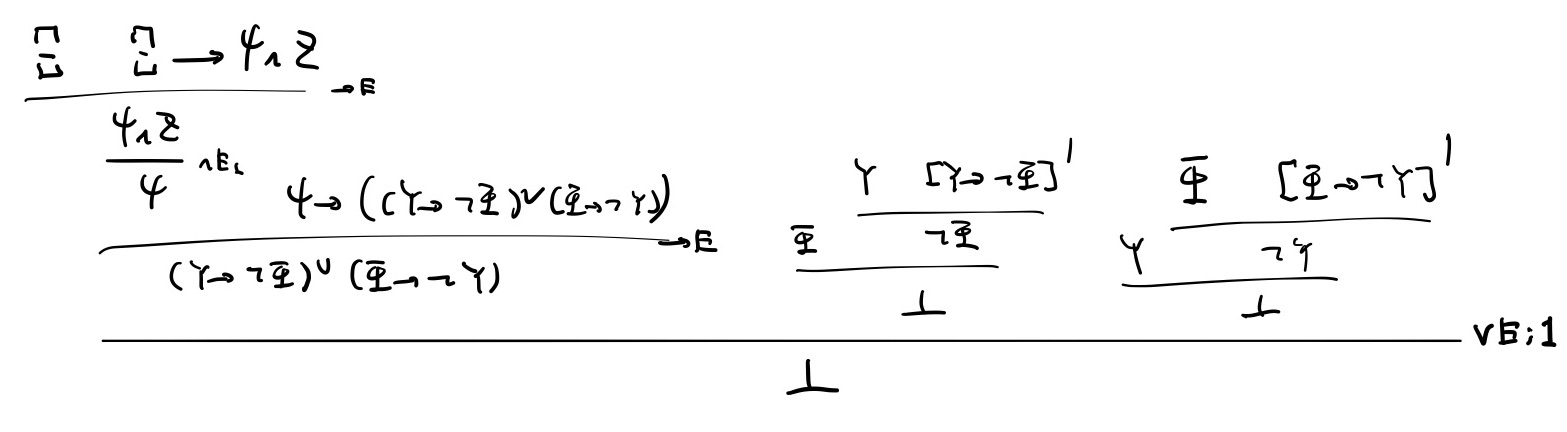
\includegraphics[width=15cm]{figure9.jpg}
    \end{center}
    部分証明図$\frac{[C]}{\bot}\Pi_4$は次の通りである.
    \begin{center}
        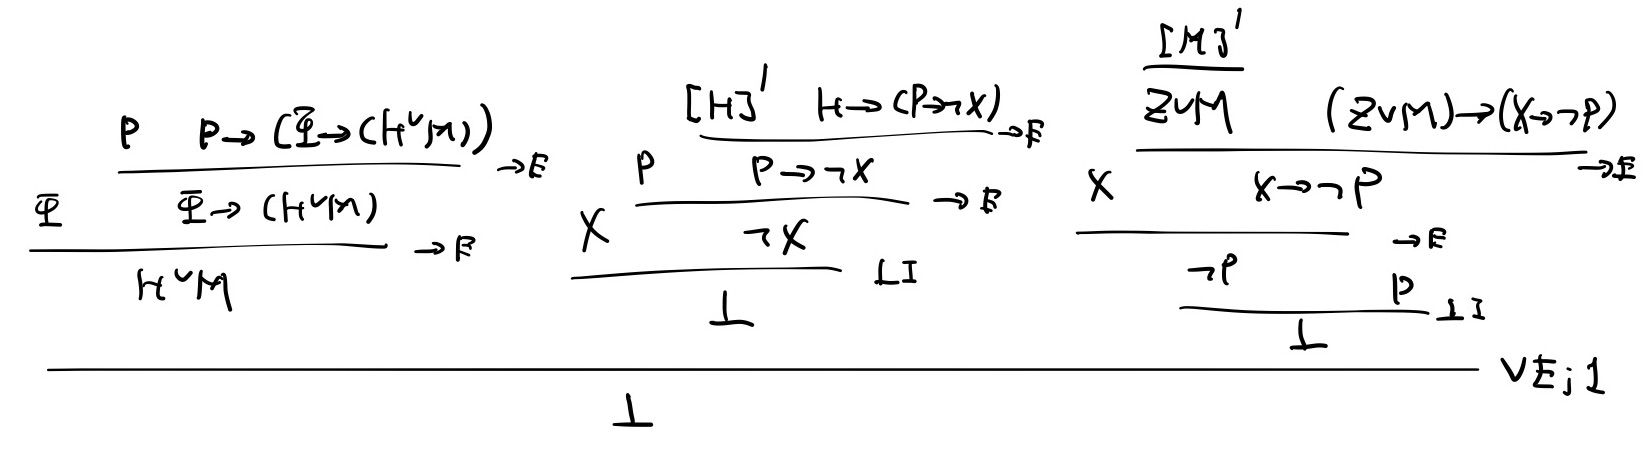
\includegraphics[width=15cm]{figure10.jpg}
    \end{center}
    部分証明図$\frac{[D]}{\bot}\Pi_5$は次の通りである.
    \begin{center}
        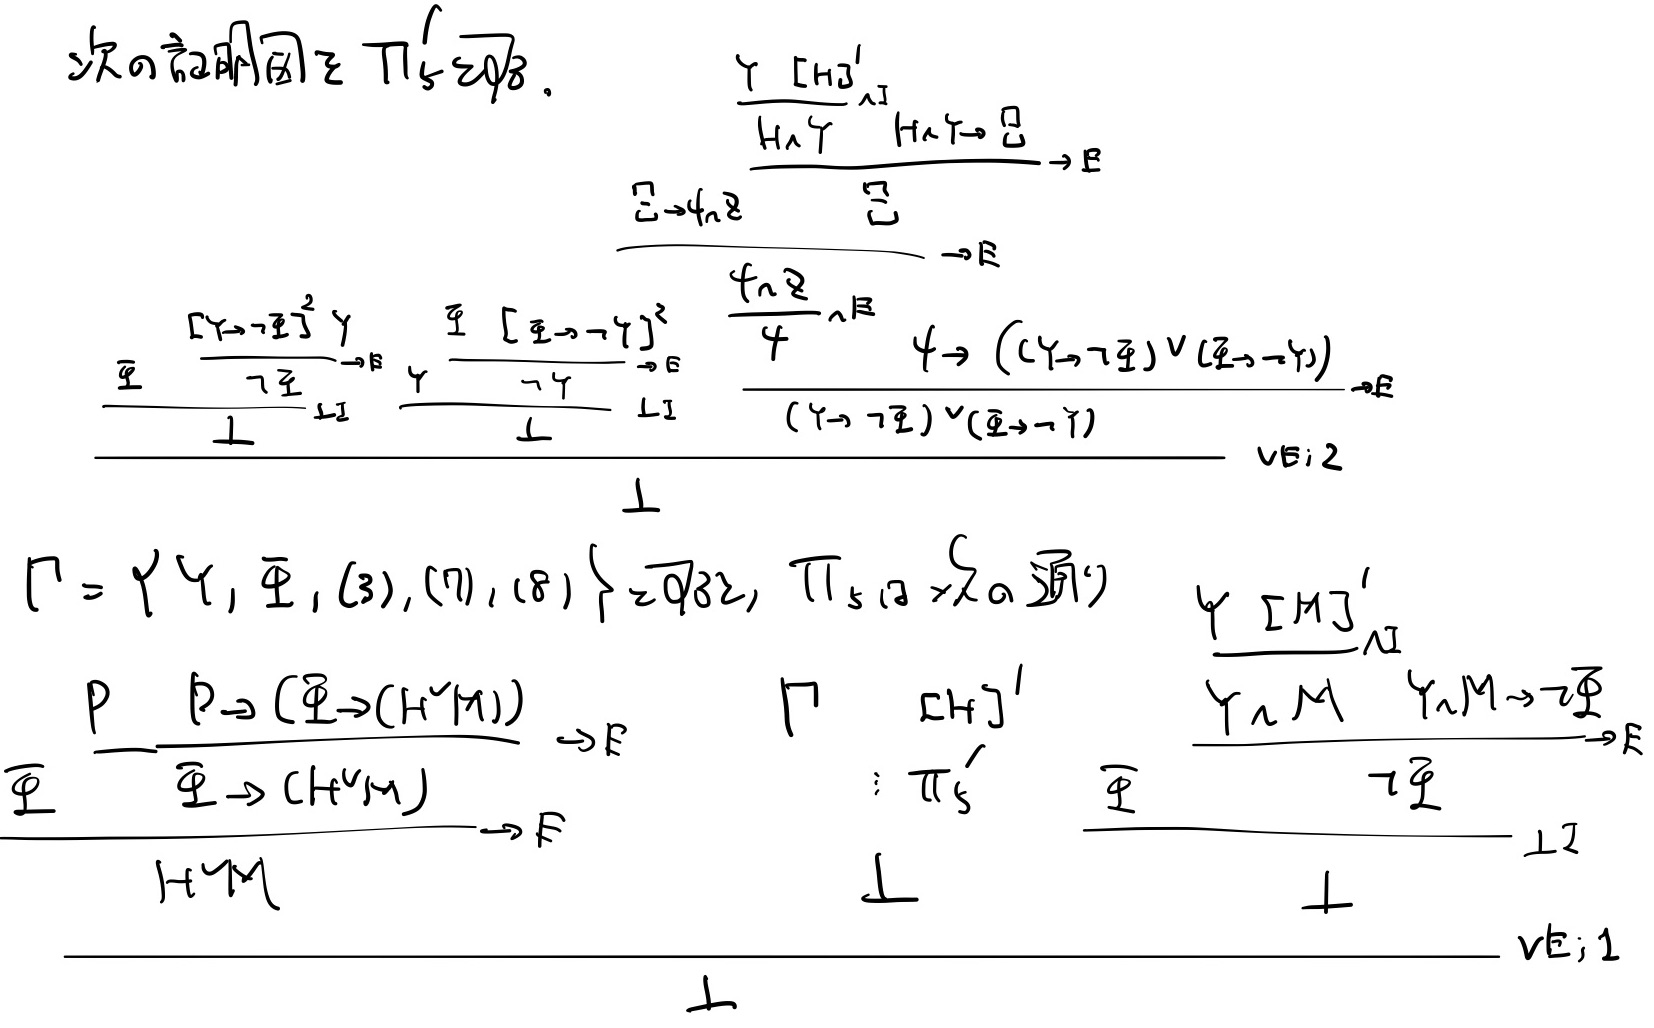
\includegraphics[width=15cm]{figure11.jpg}
    \end{center}
    以上$\Pi_1,\cdots,\Pi_5$を用いて,命題$[*]$の証明図は$\Gamma_2:=\{(3),(10)\},\;\Gamma_3:=\{(3),(7)\},\;
    \Gamma_4:=\{(4),(5),(6)\},\;\Gamma_5:=\{(3),(4),(7),(8),(9)\}$として次のように表せる.
    \begin{center}
        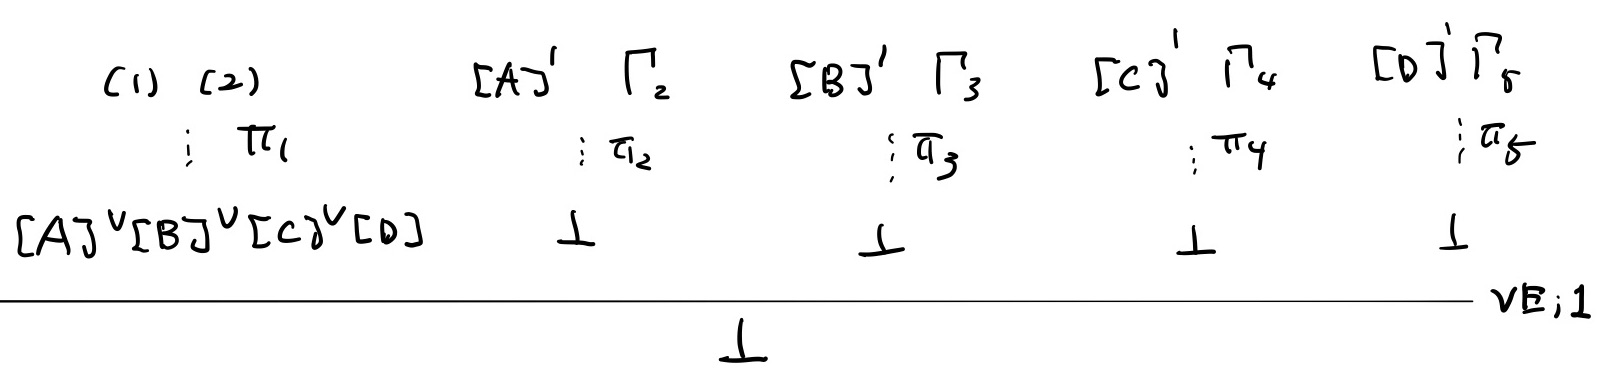
\includegraphics[width=15cm]{figure12.jpg}
    \end{center}
\end{proof}

\section{}

\begin{notation*}
    PAの言語を$\mathrm{L(PA)}=\{0,S,+,\cdot,=\}$とする.ただし,慣習に従って$x\cdot y$は$xy$とも書くこととする.
\end{notation*}

\begin{problem}
    次の命題[\#]をPA!の閉論理式に書き換えよ.
    \begin{quote}
        [\#] いかなる自然数$x$と、$1\le y$かつ$y\le x$であるようないかなる自然数$y$についても、$y$は、$x$の階乗$x!$の約数である。
    \end{quote}
\end{problem}
\begin{proof}[\bf{[解]}]
    \[ \forall x\forall y\;(1\le y\land y\le x\to\exists z(x!=y\cdot z)) \]
    を,さらに$1,\le\notin\mathrm{L(PA)}$の略記を展開して
    \[ \forall x\forall y\;(\exists z_1(S0+z_1=y)\land\exists z_2(y+z_2=x)\to\exists z(x!=y\cdot z)) \]
\end{proof}

\begin{problem}
    次の補助定理1を示せ.
    \begin{quote}
        [補助定理1]$\forall y\forall z\;(y+z=0\to (y=0\land z=0))$
    \end{quote}
\end{problem}
\begin{proof}[\bf{[解]}]
    論理式$x+y=0\to(x=0\land y=0)$を$\Phi(x,y)$と略記する.
    先ず,自由変項$x$について,$\forall y\;\Phi(x,y)$の証明図$\Pi'$は次の通りである.
    \begin{center}
        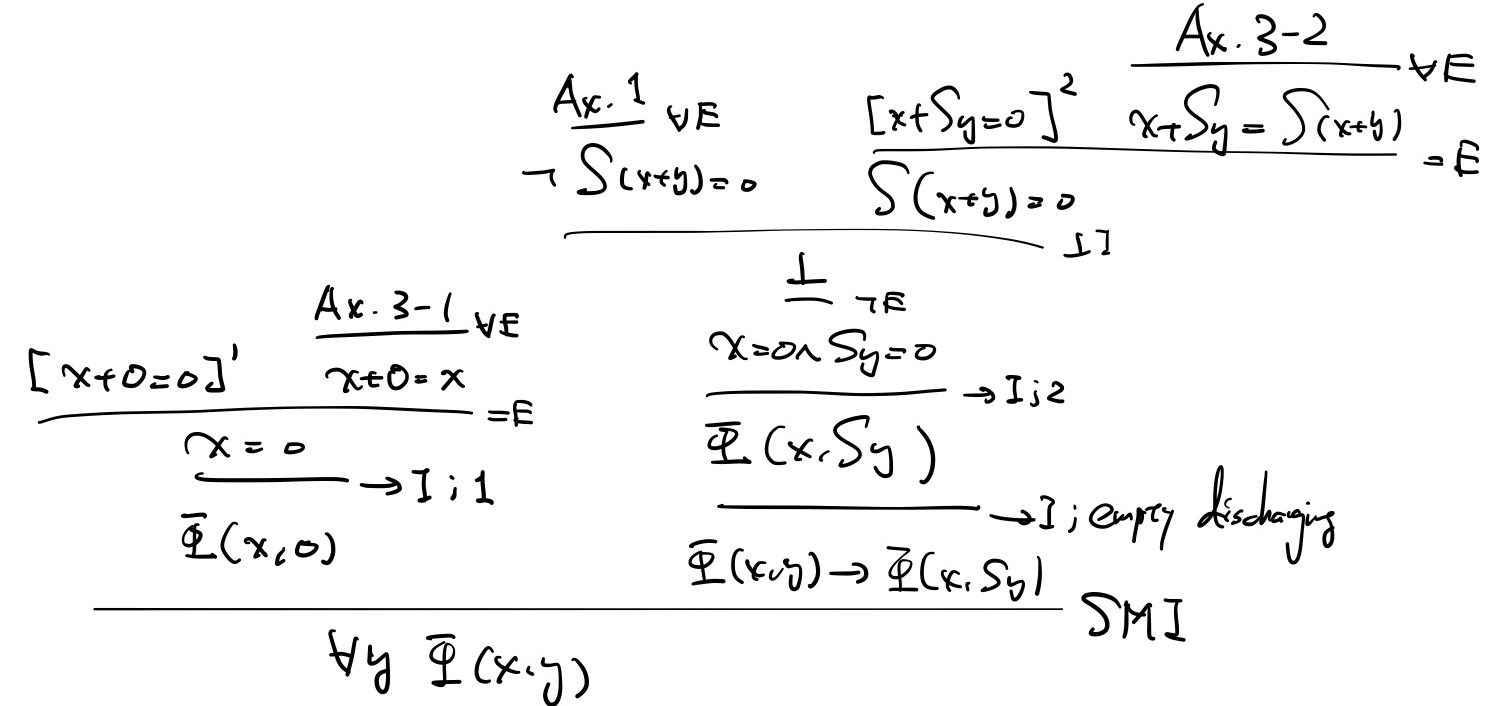
\includegraphics[width=15cm]{figure3-1.jpg}
    \end{center}
    これを用いて$\forall y\;\Phi(x,y)$を$\Psi(x)$と略記すると,
    $\forall x\;\Psi(x)$の証明図は次の通り.
    \begin{center}
        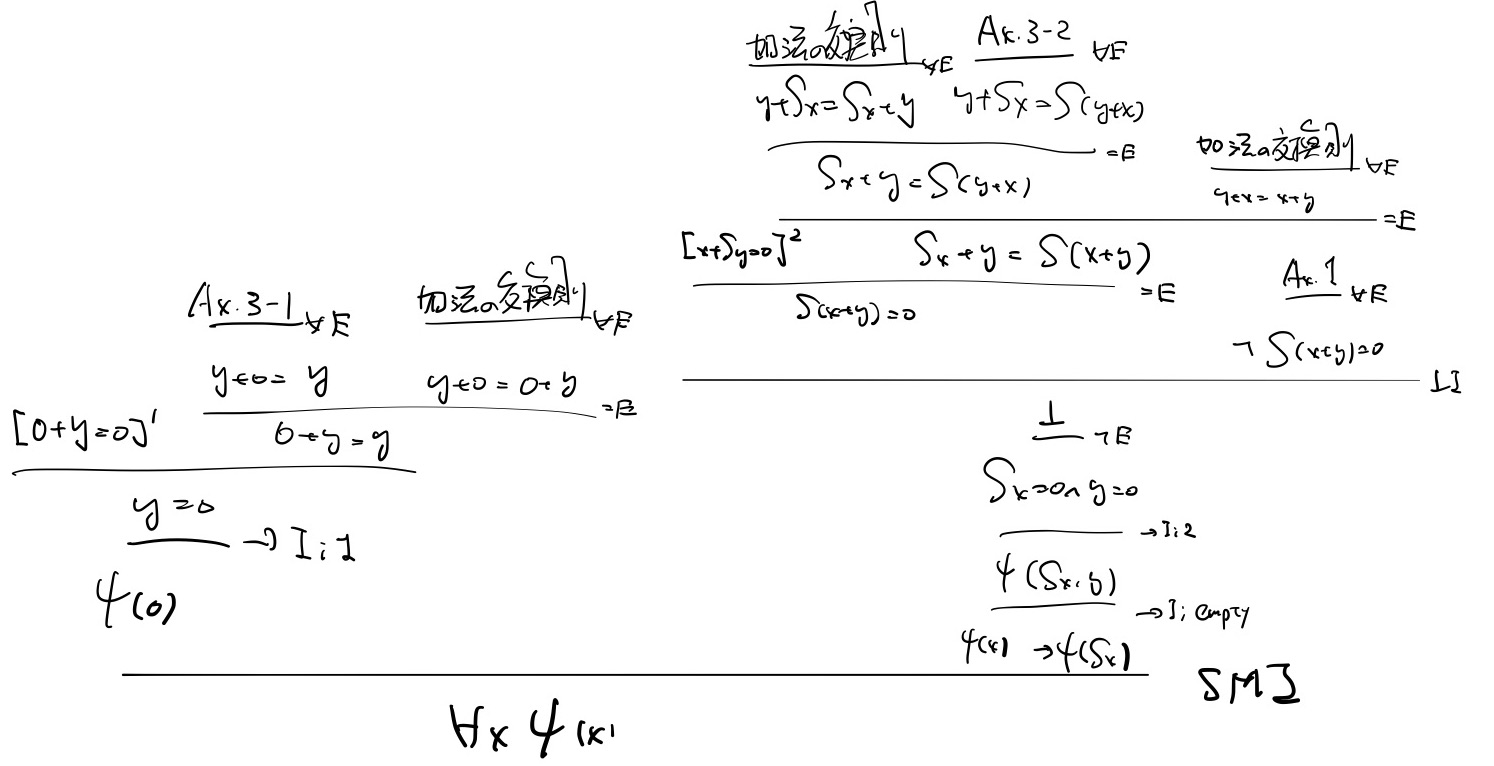
\includegraphics[width=15cm]{figure3-2.jpg}
    \end{center}
\end{proof}

\begin{problem}
    次の補助定理2を示せ.
    \begin{quote}
        [補助定理2]いかなる自然数$x$と$y$についても、もしも$y\le Sx$ならば、$y=Sx\lor y\le x$である:
        $\forall x\forall y\;(\exists z(y+z=Sx)\to (y=Sx\lor\exists z'(y+z'=x)))$
    \end{quote}
\end{problem}
\begin{proof}[\bf{[解]}]
    分離可能性の定理$\vdash_{PA}z=0\lor\exists z'(z=Sz')$より$z=0$と$\lnot z=0$の場合で場合分けすることによる証明の証明図は次の通りになる.ただし,$x,y,z$は互いに異なる変数とする.
    \begin{center}
        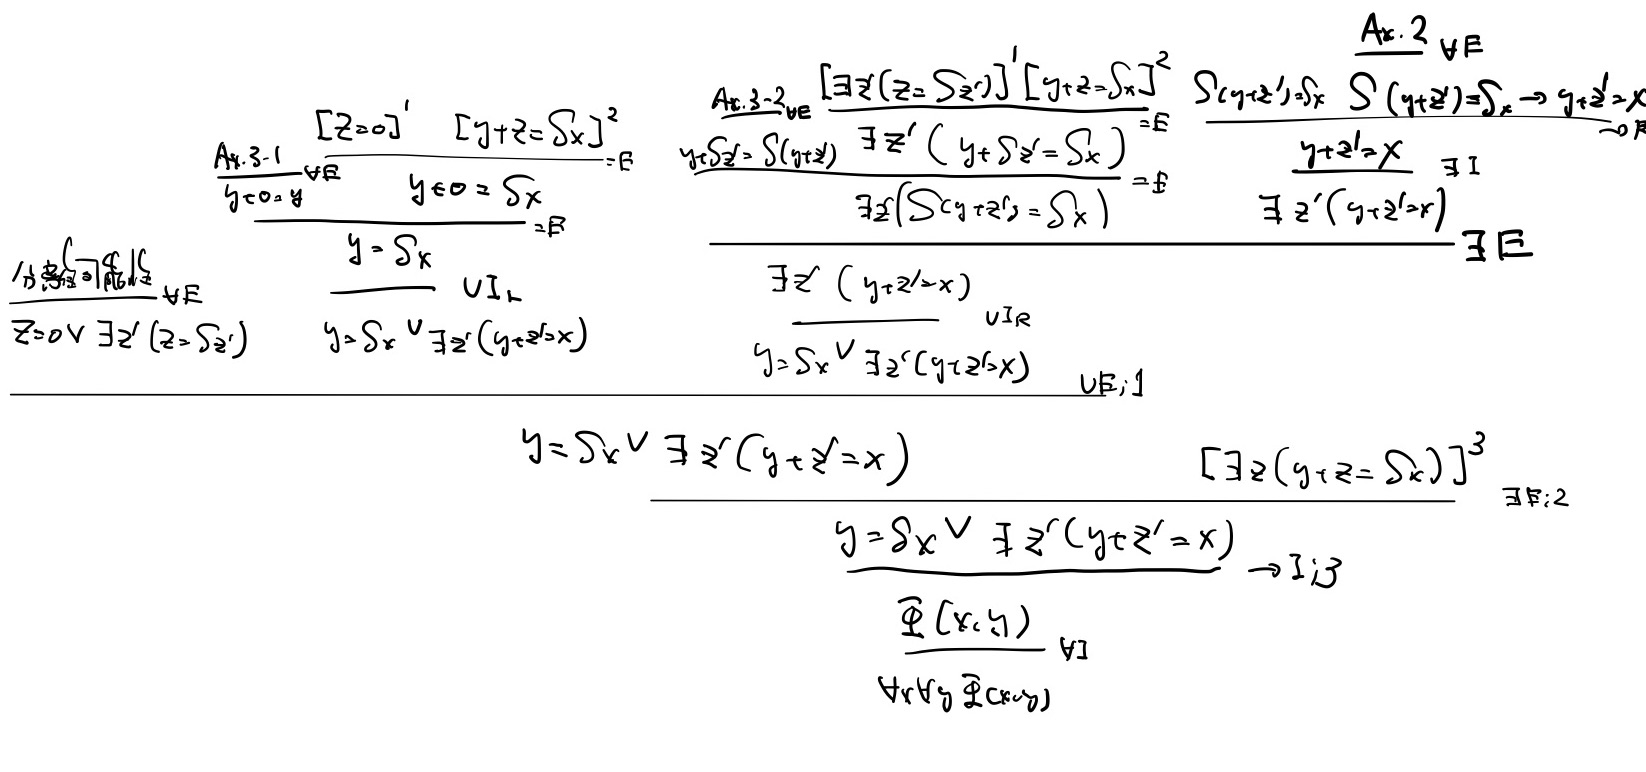
\includegraphics[width=15cm]{figure3-3.jpg}
    \end{center}
\end{proof}

\begin{problem}
    定理[\#]を示せ.
\end{problem}
\begin{proof}[\bf{[解]}]
    命題$\exists z_1(S0+z_1=y)\land\exists z_2(y+z_2=x)\to\exists z(x!=yz)$を$\phi_1(x,y)\land\phi_2(x,y)\to\phi_3(x,y)$または$\Phi(x,y)$と書く.
    また,簡明さのために,所々2つの推論を1つの横棒のみと2つの注記を用いて$\frac{\cdots}{\cdots}\land E_L,\land E_R$などと略記した.
    部分証明図$\Pi_1$を次のとおりとする.
    \begin{center}
        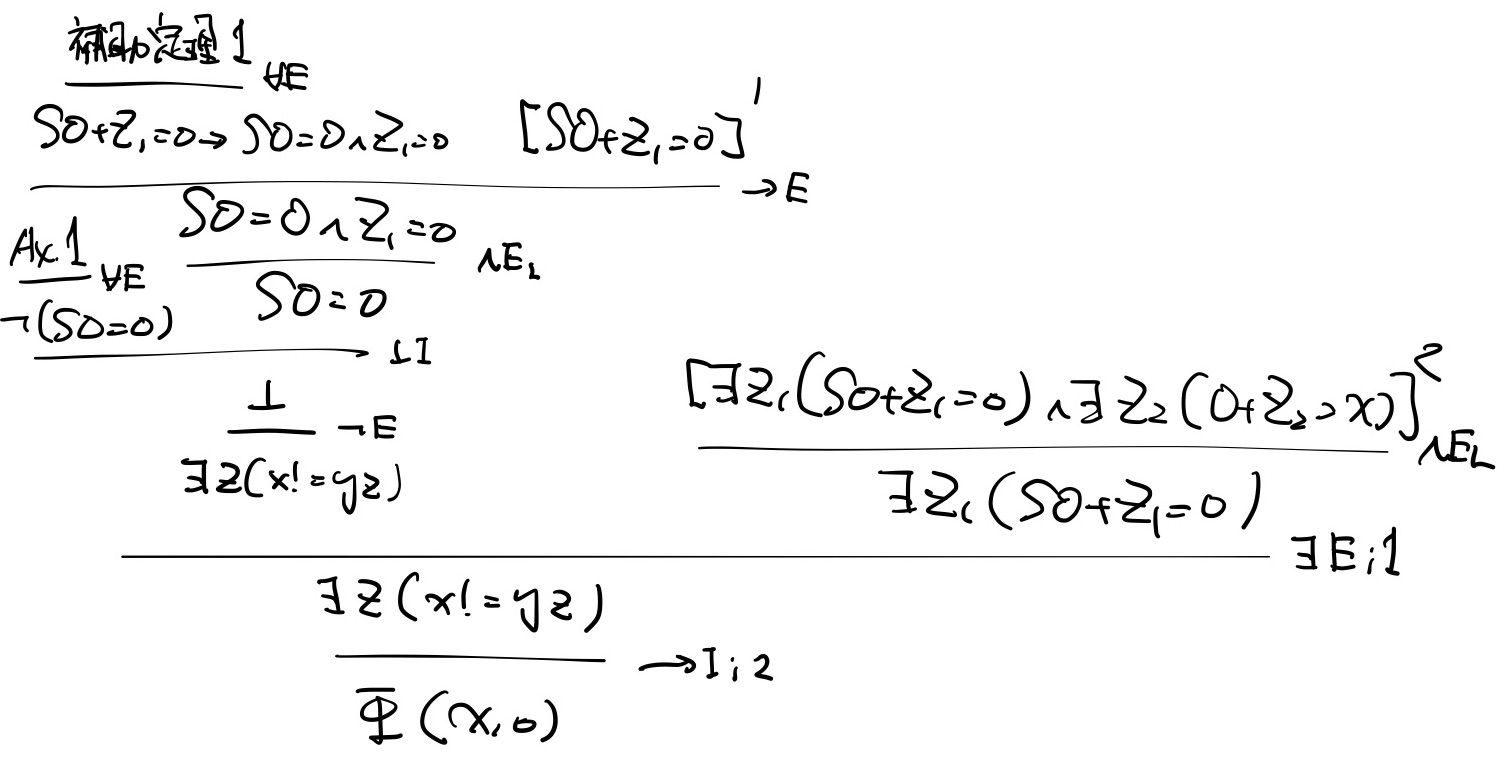
\includegraphics[width=15cm]{figure3-4.jpg}
    \end{center}
    部分証明図$\Pi_2$を次のとおりとする.
    \begin{center}
        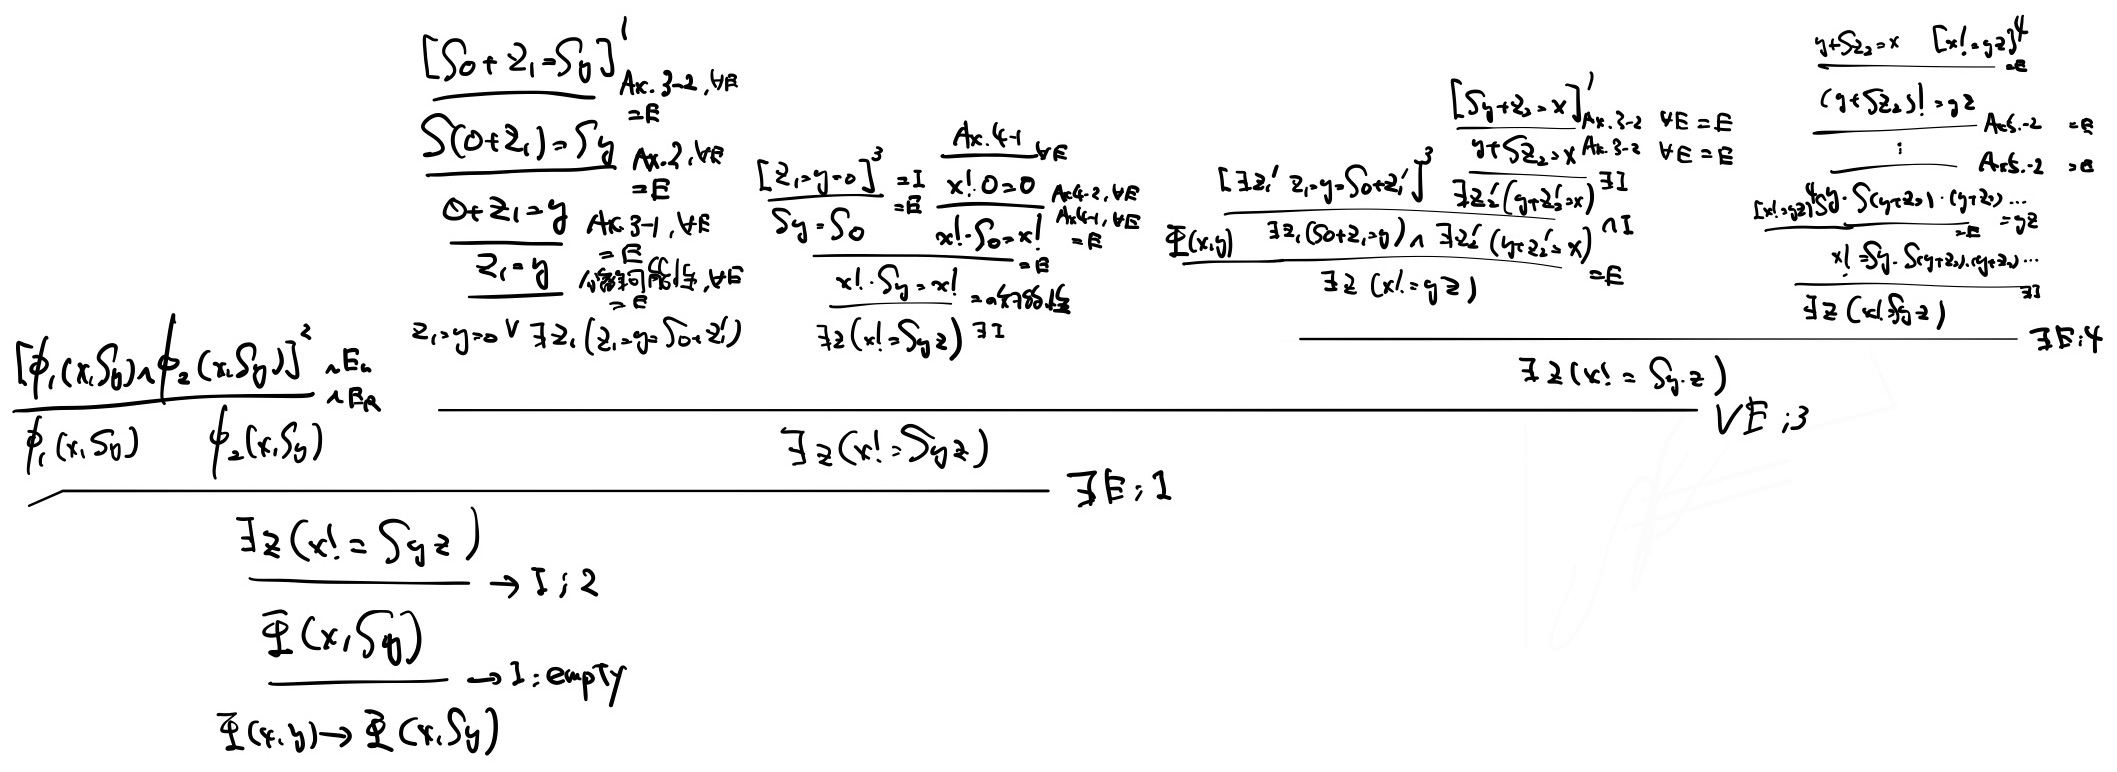
\includegraphics[width=15cm]{figure3-5.jpg}
    \end{center}
    以上の部分証明図$\Pi_1,\Pi_2$を用いて,$\forall y\Phi(x,y)$の証明図は次の通りになる.ただし,$\Gamma_1=\{\mathrm{Ax.1}, 補助定理1 \},\Gamma_2=\{\mathrm{Ax.2,Ax.3-1,Ax.3-2,Ax.4-1,Ax.4-2,Ax.5-2},分離可能性,=の対称性\}$と置いた.
    \begin{center}
        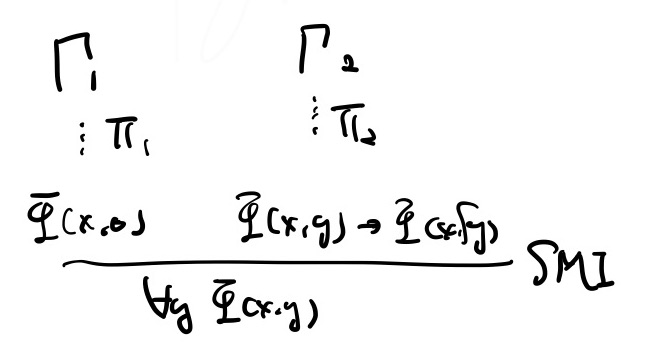
\includegraphics[width=15cm]{figure3-6.jpg}
    \end{center}
    次に,論理式$\forall y\Phi(x,y)$を$\Psi(x)$と書く.次を部分証明図$\Sigma_1$とする.
    \begin{center}
        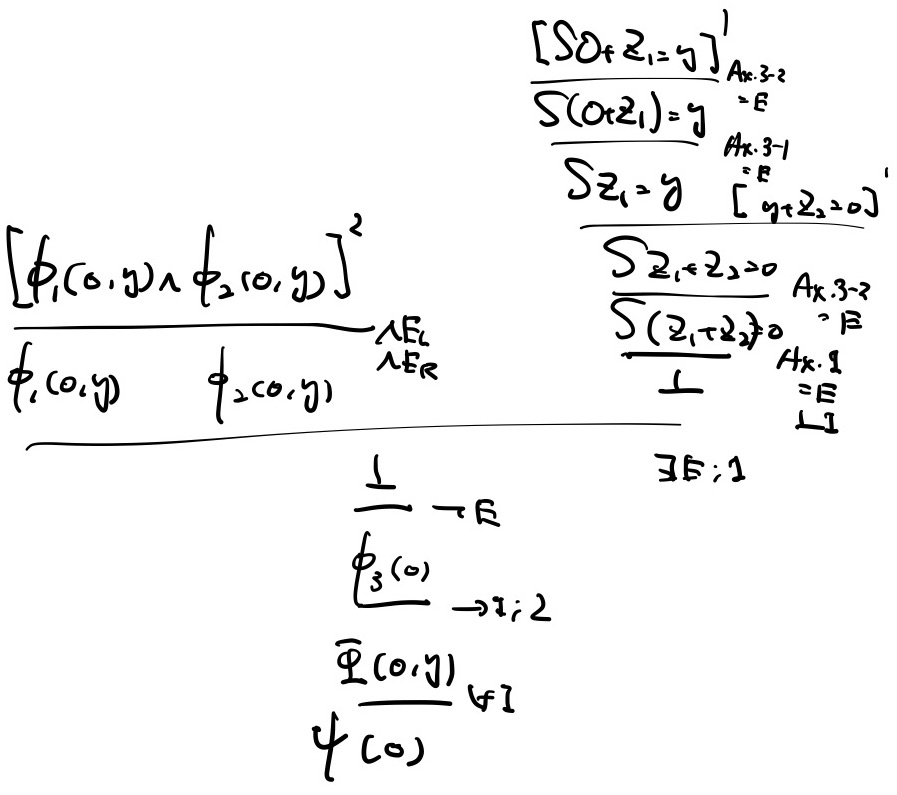
\includegraphics[width=15cm]{figure3-7.jpg}
    \end{center}
    次を部分証明図$\Sigma_2$とする.
    \begin{center}
        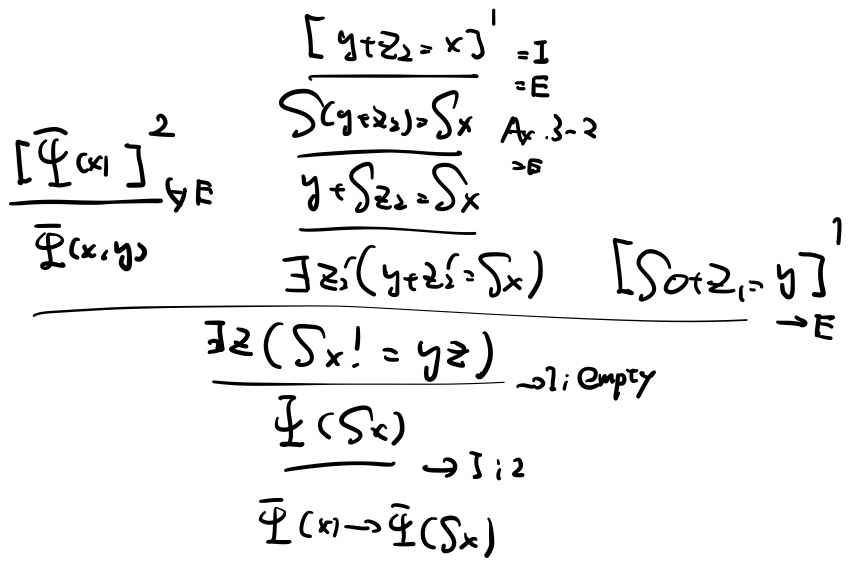
\includegraphics[width=15cm]{figure3-8.jpg}
    \end{center}
    以上を用いて,$\forall x\Psi(x)$の証明図は次の通り.ただし,$\Gamma'_1=\{\mathrm{Ax.1,Ax.3-1,Ax.3-2 }\},\Gamma'_2=\{\mathrm{Ax.3-2}\}$と置いた.
    \begin{center}
        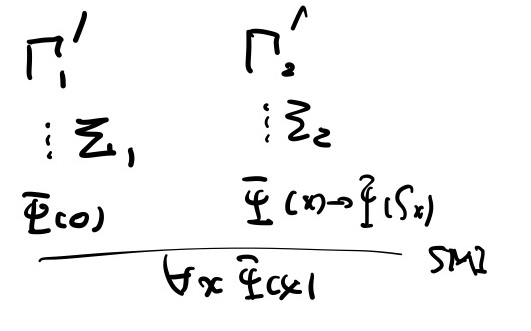
\includegraphics[width=15cm]{figure3-9.jpg}
    \end{center}
\end{proof}

\section{}

\begin{notation*}
    順序集合論の言語に$\le$は含まれているものとする.また,$\lnot(u\in Q)$を$u\notin Q$と略記する.
\end{notation*}

\begin{problem}
    次の定理を一階の閉論理式で表せ.ただし,$(S,\le)$を順序集合,$(Q,\le)$をその部分順序集合とする.
    \begin{quote}
        [\%] もしも$x$、$y$が、互いに等しくない(つまり、$\lnot x=y$であるような)$Q$の極大元だとすると、そのとき、$S$のいかなる元$u$についても、もしも$u$が$Q$の上限ならば、$u$は$Q$の元ではない。
    \end{quote}
\end{problem}
\begin{proof}[\bf{[解]}]
    \begin{align*}
        &(\exists x\in Q \exists y\in Q (\forall z\in Q(x\le z\to x=z)\land \forall z\in Q(y\le z\to y=z)\land x\ne y))\\
        \to& (\forall u\in S((\forall t\in Q (t\le u)\land \forall s\in S(\forall t\in Q t\le s\to u\le s))\to u\notin Q))
    \end{align*}
\end{proof}

\begin{problem}\mbox{}
    [\%]を示せ.
\end{problem}
\begin{proof}[\bf{[解]}]\mbox{}
    [\%]を$\exists x\in Q\exists y\in Q\Phi(x,y)\to\exists u(\phi_1\to u\notin Q)$と表す.即ち,$\forall z\in Q(x\le z\to x=z)\land \forall z\in Q(y\le z\to y=z)\land x\ne y$を$\Phi(x,y)$,$\forall t\in Q(t\le u)\land \forall s\in S(\forall t\in Q t\le s \to u\le s)$を$\phi$と表した.
    すると,証明図は以下の通りである.
    \begin{center}
        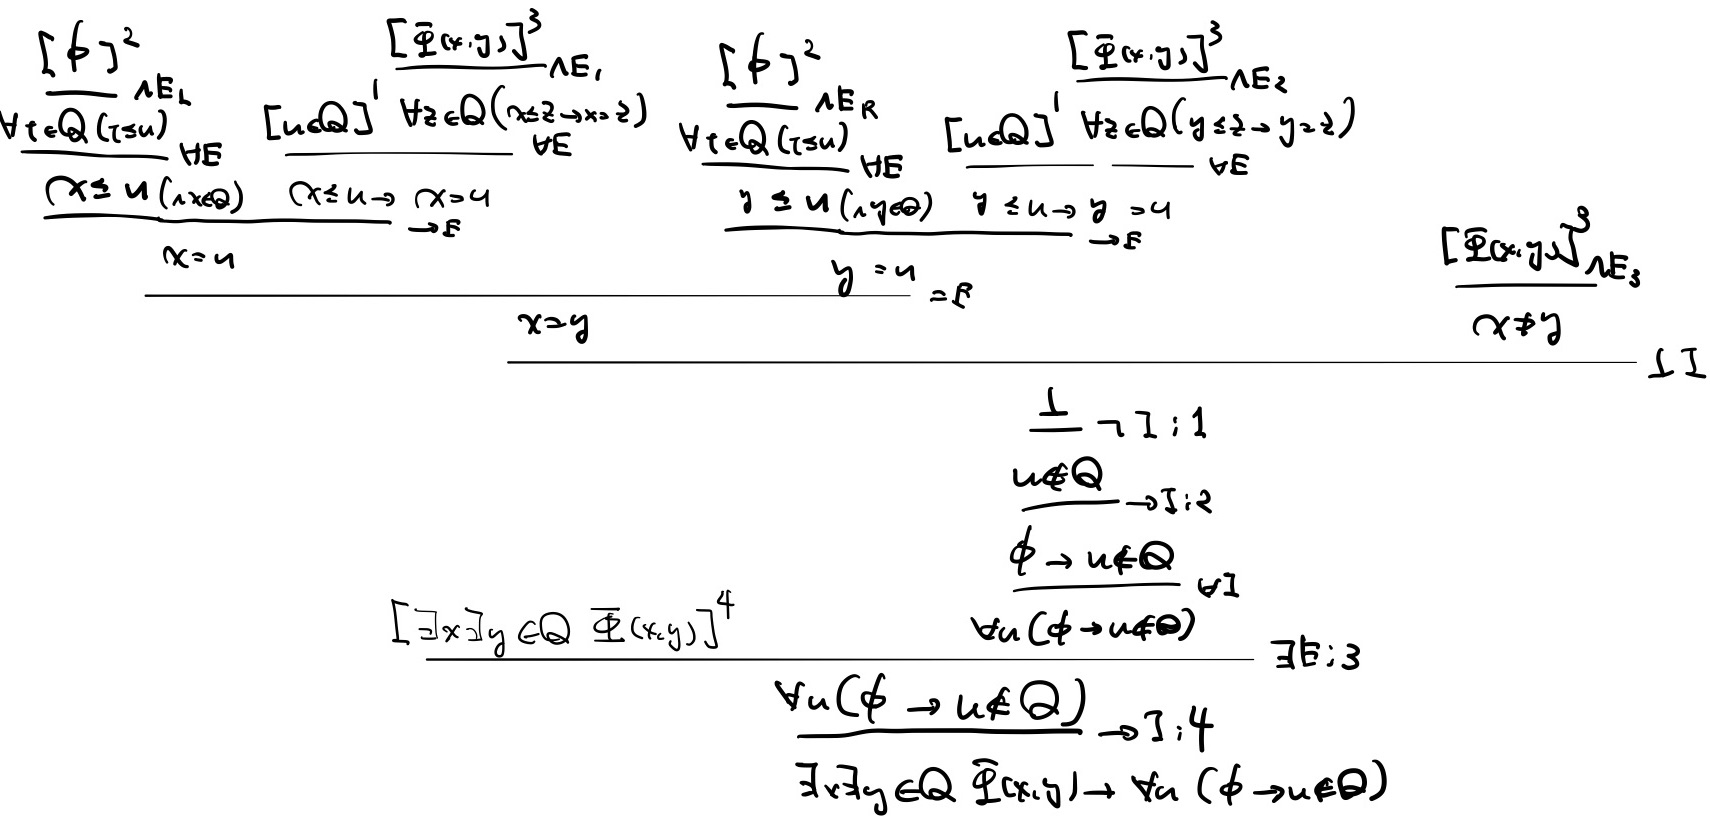
\includegraphics[width=15cm]{figure4-1.jpg}
    \end{center}
\end{proof}

\section{}

\begin{problem}
    記号論理学に関わる何らかの証明、または証明の解説を書け。
\end{problem}
筆者は数学への動定理証明システムの応用(またはその逆)に興味を持っている.
そこで,記号論理学の授業の内容に関連して,
以降小節に分けて,証明論における定理であるHerbrandの定理とその証明を示す.

\subsection{一階述語論理に構文論についての準備:Skolem標準形}

\begin{notation}\mbox{}
    \begin{enumerate}
        \item 以降言語$L$を1つ固定し,変項を$x,y,z,\cdots$,言語$L$に含まれる定数を$a,b,c,\cdots$,述語を$P,Q,R,\cdots$と書くこととする.
        \item Prologでの記法に倣い,述語のarity $n\in\N$を$P/n$というように述語記号に/を挟んで添えて書く.
        \item $L$の有限列として一致するという同値関係を$\equiv$で表す.
        \item $:\Leftrightarrow$は,左辺を右辺で定義すると言うメタ言語内での記法である.
        \item 同様にして,$\Rightarrow$や$\Leftrightarrow$はメタ論理での「ならば」記号として使い,$\to$や$\leftrightarrow$を一階述語論理の論理記号として採用する.
        \item 変数や定数の組を$\vec{x}:=(x_1,\cdots,x_n)$と書き,$\forall\vec{x}$を記号列$\forall x_1\forall x_2\cdots\forall x_n$の略記とする.
    \end{enumerate}
\end{notation}
\begin{remark}
    また,文献\cite{新井敏康}に沿って,一階論理で使われる記号のうち,非論理記号の集合のことを言語$L$とする流儀を採用した.
\end{remark}

\begin{definition}[term]
    \textbf{L-項}全体の集合$Tm_L$を次のように帰納的に定める.
    \begin{enumerate}
        \item  $x,y,z,\cdots,a,b,c,\cdots\in Tm_L$である.
        \item  $f:Tm_L^n\to Tm_L\;\;\;(f/n\in L)$について,$x_1,x_2,\cdots,x_n\in Tm_L$である時に$f(x_1,x_2,\cdots,x_n)\in Tm_L$である.
        \item 以上の1と2により$Tm_L$の元であるとわかるもののみをL-項と定義する
    \end{enumerate}
    変数$x,y,z,\cdots$を含まないL-項を\textbf{L-閉項(L-closed term)}/または\textbf{L-基礎項(L-ground term)}と言う.
\end{definition}
\begin{definition}[literal]
    次のいずれかの形をした論理式を,\textbf{原子論理式(atomic formulta)}と言う.
    \begin{align*}
        t_1 &= t_2, & R(t_1,\cdots,t_n), && (t_i\in Tm_L, R/n\in L).
    \end{align*}
    原子論理式とその否定形を\textbf{literal}と言う.
\end{definition}

\begin{definition}[formula]
    \textbf{L-論理式}とは,次のように帰納的に定義される記号列のことである.
    \begin{enumerate}
        \item literalは論理式である.
        \item 論理式$\varphi,\psi$について,$(\varphi\lor\psi),\;(\varphi\land\psi),\;(\varphi\to\psi)$は論理式である.
        \item 論理式$\varphi$と変数$x$について,$(\exists x\varphi),\;(\forall x\varphi)$は論理式である.
    \end{enumerate}
    L-論理式全体の集合を$Fml_L$と書くこととする.
\end{definition}

以降,一般のL-論理式についてではなく,次の2種の標準形のみに議論を絞る.

\begin{definition}[prenex normal form]
    次の形の論理式を\textbf{冠頭標準形}の論理式という.
    \[ Q_1x_1\cdots Q_nx_n\theta\;\;\;(n\ge 0,Q_i\in\{\exists,\forall\},\theta には量化記号なし) \]
    この時$\theta$をこの論理式の母式(matrix)という.
\end{definition}

\begin{definition}[Skolem normal form]
    冠頭標準形の論理式$\varphi$について,$\varphi$中の各存在量化記号$\exists y_l\;(l\in\N)$について,それより前に全称量化記号が$n_l$個$\forall x_1^l,\cdots,\forall x_{n_l}^l$とあるとすれば,
    $n_l$-変数の新たな関数記号$f_l$を導入して,$\varphi$の母式中の変数$y_l$を$f_l(x^l_1,\cdots,x^l_{n_l})$で置き換えることで,存在量化記号$\exists y_l$を消去することができる.これは拡張された言語$L\cup\{f_i\}$での$\forall$-論理式であり,これを\textbf{Skolem(連言)標準形}という.
\end{definition}
次が成り立つという意味で,これは標準形である.
\begin{proposition}\label{prop-1}
    冠頭標準形の論理式$\varphi$のモデルに対して,適切にSkolem関数記号$f_i$に解釈を追加することでそのSkolem標準形$\varphi^S$のモデルが得られ,
    $\varphi^S$のモデルからSkolem関数への解釈を削れば$\varphi$のモデルが得られる.
\end{proposition}
確かに,$\varphi$での各存在量化子で縛られた変数$y_l$に対して,
$y_l$が存在することとSkolem関数$f_l$が構成可能であることに等価である.

\subsection{一階述語論理の意味論についての準備:充足可能性}

\begin{definition}[structure]
    \textbf{L-構造}とは,議論領域$M\ne\varnothing$と解釈写像$F:L\to M$との対$\mathcal{M}:=(M,F)$であって,言語$L$に対して次を満たすもののことである.
    \begin{enumerate}
        \item $R/n\in L$に対して,$F(R)=:R^\mathcal{M}$は$M$上のn-項関係である:$R^\mathcal{M}\subset M^n$.
        \item $f/n\in L$に対して,$F(f)=:f^\mathcal{M}$は$M$上のn-項関数である:$f^\mathcal{M}:M^n\to M$.
        \item 特に定数$c\in L$に対しては,$F(c)=:c^\mathcal{M}\in M$である.
    \end{enumerate}
    構造$\mathcal{M}$は通常$\mathcal{M}=(M;R^\mathcal{M},\cdots,f^\mathcal{M},\cdots,c^\mathcal{M},\cdots)$と表し,$|\mathcal{M}|:=M$を構造$\mathcal{M}$の対象領域もしくは領域(universe)という.
\end{definition}
\begin{remark}
    数学の慣習では,右肩の添字を省略し,構造$\mathcal{M}$と領域$M$を混用する.例えば$G=(G,+,-,0)$など.
\end{remark}

構造中心に論理式をみる場合,これに対応して言語を拡張する操作を定義しておきたい.
言語$L$とL-構造$\mathcal{M}=(M,F)$が与えられた時,これに適して言語$L$を拡張した言語を$L(\mathcal{M}):=L\cup\{c_a\mid a\in M\}$
と定める.この$c_a$を$a\in M$の名前(name)という.解釈写像$F:L\to M$は自然に$F:L(\mathcal{M})\to M$に拡張される.

\begin{definition}[value of terms]
    $L$を言語,$\mathcal{M}=(M,F)$をL-構造,$t$を$L(\mathcal{M})$-閉式とする.
    解釈写像$F$が定める式$t$の\textbf{値}$t^\mathcal{M}$を次のように帰納的に定める.
    \begin{enumerate}
        \item $t/0$ならば,$t^\mathcal{M}:=c^\mathcal{M}$.
        \item $\exists f\in L,\; t/n\equiv f(t_1,\cdots,t_n)$ならば,$t^\mathcal{M}:=f^\mathcal{M}(t^\mathcal{M}_1,\cdots,t^\mathcal{M}_n)$.
    \end{enumerate}
\end{definition}

\begin{definition}[satisfication relation]
    $L$を言語,$\mathcal{M}=(M,F)$をL-構造,$\varphi$を$L(\mathcal{M})$-文とする.
    L-構造と$L(\mathcal{M})$-閉論理式の\textbf{充足関係}$\vDash$を,次のように帰納的に定義する.
    なお,7,8の定義の右辺はメタ論理を一階の言語で表現した文章である.
    \begin{enumerate}
        \item $\mathcal{M}\vDash(t_1=t_2):\Leftrightarrow t^\mathcal{M}_1=t_2^\mathcal{M}$.
        \item $\mathcal{M}\vDash R(t_1,\cdots,t_n)\;(R\in L):\Leftrightarrow (t_1^\mathcal{M},\cdots,t_n^\mathcal{M})\in R^\mathcal{M}$.
        \item $\mathcal{M}\vDash\lnot\varphi:\Leftrightarrow\mathcal{M}\nvDash\varphi:\Leftrightarrow\mathcal{M}\vDash\varphi$でない.
        \item $\mathcal{M}\vDash\varphi\lor\psi:\Leftrightarrow\mathcal{M}\vDash\varphi\lor\mathcal{M}\vDash\psi$.
        \item $\mathcal{M}\vDash\varphi\land\psi:\Leftrightarrow\mathcal{M}\vDash\varphi\land\mathcal{M}\vDash\psi$.
        \item $\mathcal{M}\vDash\varphi\to\psi:\Leftrightarrow\mathcal{M}\vDash\varphi\to\mathcal{M}\vDash\psi\Leftrightarrow\lnot(\mathcal{M}\vDash\varphi)\lor\mathcal{M}\vDash\psi$.
        \item $\mathcal{M}\vDash\exists v(v),\;\varphi:\Leftrightarrow\exists a\in M,\; \mathcal{M}\vDash\varphi(c_a)$.
        \item $\mathcal{M}\vDash\forall v(v),\;\varphi:\Leftrightarrow\forall a\in M,\; \mathcal{M}\vDash\varphi(c_a)$.
    \end{enumerate}
\end{definition}

\subsection{Herbrandの定理}
\begin{screen}
Herbrandの定理とは,
Jacques Herbrandが1930年に提出した証明論に於ける定理であり,
一階述語論理の論理式の充足不能性(または恒真性)の判定を,Herbrand基底上の有限回の命題論理の充足不能性の判定に還元する定理である.
一階述語論理と命題論理の充足不能性の意味論的定義は全く異なり,後者に於ける充足不能性
は各Herbrand基底に対する真理値の付与の仕方について
有限回の機械的な操作で判定可能である.
従って,この定理が以降自動定理証明システム開発に当たっての理論的基盤となった.
なお,Herbrand定理が与えられたからと言って,実際に直接的に証明を構成する,
または充足可能性/不能性を実用的な範囲での制限時間内で判定する(ようなアルゴリズムを与える)という課題は極めて困難で,
論理プログラミング言語として代表的なPrologの誕生は1965年のJohn Alan Robinson
による導出原理の提出の仕事を待たねばならない.
また,Prologも,扱う一階述語論理の論理式に強い制約をつけたものになっている.
自動定理証明システムの開発はまだまだこれからである\footnote{一切の制約のない一般の一階述語論理の論理式の恒真性の判定問題は,Turing機械の非停止性の認識問題に帰着されるため,決定不能であることはすでに知られている.}.
\end{screen}

先ず,Herbrandの定理は,
一階述語論理の意味論と命題論理の意味論の接続にあたって,
特別な構造「Herbrand構造」を用意する.
これはHerbrand基底と呼ばれるL-原子論理式を命題変数として,
一階述語論理のL-論理式を命題論理的な意味論の世界へ解釈するようなL-構造である.
このことを見ていく.

\begin{definition}[Herbrand universe]
    L-論理式$A$の\textbf{エルブラン領域}とは,言語Lの記号のうち,次の当てはまるものからなる部分集合$L_A$から生成される$L_A$-閉項全体$Tm_{L_A}$のことをいう.
    \begin{enumerate}
        \item $A$に出現する定数記号
        \item $A$に自由出現する変数記号
        \item $A$に出現する関数記号
    \end{enumerate}
    ただし,$A$に1も2も存在しない場合は,定数記号を$L$から自由に1つ選んで$L_A$の元とする.
\end{definition}
\begin{remark}
    具体的に取れる点の全体領域/閉包を確保したことになる.
\end{remark}

\begin{definition}[Herbrand structure]
    L-論理式$A$の\textbf{Herbrand構造}とは,Herbrand領域$Tm_{L_A}$を領域とし,
    その上のL-閉項を次のように解釈する写像$F_{Tm_{L_A}}$を解釈写像とする
    構造$\M_{L_A}:=(L_A,\id_{Tm_{L_A}})$のことである.
    解釈写像$F_{Tm_{L_A}}$は,$L_A$に属する記号はそれ自身に,即ち$Tm_{L_A}$の元はそれ自身に写し,
    述語記号$P/n\in L$は,
    勝手な関数$(L_A)^n\to\{\top,\bot\}$に写す(従って述語記号の解釈は各Herbrand構造について異なり得る)ものとする.
    また,論理記号は命題論理の結合子として解釈する.
\end{definition}
\begin{definition}[Herbrand-satisfiable]
    論理式(の集合)が\textbf{Herbrand充足可能}であるとは,その論理式(の集合)を充すHerbrand構造が存在することをいう.
\end{definition}

\begin{proposition}
    Skolem標準形の論理式は,充足可能ならばHerbrand充足可能である.
    逆は自明に成り立つから,即ちSkolem標準形の論理式にとって,充足可能性とHerbrand充足可能性とは同値である.
\end{proposition}
\begin{proof}
    Skolem標準形の論理式$A$について,これを充足する構造$\M$が存在するとする:$\M\vDash A$.
    この構造の述語記号$P/n\in L$への解釈を,真理値関数と見た時,これが命題\ref{prop-Herbrand-magic}の方法で
    定めるHerbrand構造$\M_{L_A}$について(即ち,次の式の通りに定めた$\M_{L_A}$について),$\M_{L_A}\vDash A$である.
    \[ P^{\M_{L_A}}(t_1,\cdots,t_n) := P^\M(t_1^\M,\cdots,t_n^\M) \]
\end{proof}
\begin{example}
    論理式$\lnot P(c)\land\exists xP(x)$を考える.これは充足可能である(例えば,領域を$\{\top,\bot\}$として,そこへの解釈関数を$c\mapsto\bot,c'\mapsto\top$とし,述語$P$を適切に解釈すれば良い)
    が,Herbrand領域は論理式内にarity 1以上の関数記号が含まれないために$Tm_{L_A}=\{c\}$であり,これではHerbrand充足にはなり得ない.
    
    一方,元の論理式にSkolem関数$c'$(ここではarity 0の定数記号である)を導入してSkolem化した論理式$P(c')\land P(c)$は,言語は$L\cup\{c'\}=:L'$に拡張され,Herbrand領域は$Tm_{L'_A}=\{c,c'\}$となり,上記の証明中に示した方法で,
    充足する構造$\M$を作るたびに対応するHerbrand構造$\M_{L'_A}$も作ることができる.実際,この事実は一般化され,命題\ref{prop-Herbrand-magic}が成り立つ.
\end{example}

\begin{definition}[Herbrand basis]
    L-論理式$A$に出現する述語記号と,$A$のHerbrand領域$Tm_{L_A}$の元から作られるL-原子論理式の全体を,論理式$A$の\textbf{Herbrand基底}という.
\end{definition}
\begin{example}
    元のSkolem標準形の論理式が$\forall x\forall y(P(x)\land Q(x,f(x,c)))$である時,Herbrand基底は$\mathrm{Base}_A=\{P(c),P(f(c,c)),P(f(f(c,c),c)),\cdots,Q(c,c),Q(f(c,c),c),\cdots\}$となる.
\end{example}

\begin{proposition}[Herbrand構造と付値]\label{prop-Herbrand-magic}
    L-論理式$A$のHerbrand構造$\M_{L_A}=(L_A,\id_{Tm_{L_A}})$と,L-論理式$A$のHerbrand基底$\mathrm{Base}_{A}$上の真理値関数$\mathrm{Base}_{L_A}\to\{\top,\bot\}$とは一対一対応する.
\end{proposition}
\begin{proof}
    真理値関数$\chi_{L_A}:\mathrm{Base}_{L_A}\to\{\top,\bot\}$の値を,各述語$P/n\in L$と$L_A$-閉論理式$t_1,\cdots,t_n\in L_A$について,
    $\chi_{L_A}(P(t_1,\cdots,t_n))=P^\M(t_1,\cdots,t_n)$と定める.
    この対応付けは可逆であり,L-論理式$A$のHerbrand構造全体の集合と,集合$\mathrm{Hom}(\mathrm{Base}_{L_A},\{\top,\bot\})$上に全単射を定める.
\end{proof}

\begin{definition}[H-instance]
    Skolem標準形のL-論理式$A\equiv \forall\vec{x}A(\vec{x};\vec{a})\;(\vec{x}=(x_1,\cdots,x_n))$について,
    母式$A(\vec{x};\vec{a})$に自由出現している変数に,L-閉項を代入して得る論理式$A(\vec{t};\vec{a})$またはその有限個の連言$\land\{A(\vec{t}^i;\vec{a})\mid i\le r\}$を$A$の\textbf{例}という.
    特に,L-閉項$\vec{t}=(t_1,\cdots,t_n)$が全てHerbrand領域のものである時:$t_j\in Tm_{L_A}\;(j=1,\cdots,n)$これを\textbf{H-例}という.
    ここで,特に連言で結ばれていないH-例の全体を$\Gamma=\{A(t_1,\cdots,t_n)\mid t_1,\cdots,t_n\in Tm_{L_A}\}$と書くこととする.
\end{definition}

以上,準備が整った.まとめると次のとおりである.
\begin{itembox}[l]{Herbrand構造}
    Skolem標準形の論理式$\mathcal{A}$の母式$A(\vec{x};\vec{a})$は量化記号なしであるから,Herbrand基底$\mathrm{Base}_\mathcal{A}$の要素を命題記号(命題変数)とする命題論理式と解釈できる.
    従って,各Herbrand基底への真理値の付値$\chi_\mathcal{A}:\mathrm{Base}_\mathcal{A}\to\{\top,\bot\}$を定めるごとに,命題論理式の解釈を1つ得る.
    これは一階の論理式$\mathcal{A}$の解釈と一対一対応する.
\end{itembox}

先ず,次が成り立つ.
\begin{lemma}\label{lemma-Herbrand-first-and-zero}
    Skolem標準形のL-論理式$\A$のH-例の集合$\Gamma$が,命題論理式の集合として充足可能であるならば,$\A$は充足可能である.
\end{lemma}
\begin{remark}
    L-論理式$A$の母式を$\A$とする.$\Gamma$が命題論理式の集合として充足可能であるとする.すると,
    任意の$t_1,\cdots,t_n\in Tm_{L_\A}$に対して$A^{\M_\A}(t_1,\cdots,t_n)=\top$とするHerbrand構造$\M_\A$が存在する.
    従って命題\ref{prop-Herbrand-magic}より$\A$は充足可能である.
\end{remark}

これを用いて,Herbrandの定理を証明する.
その前に,命題論理についての基本的な結果を確認する.
\begin{theorem}[命題論理のコンパクト性定理]
    $T$を命題論理の論理式の集合とする.次の2条件は同値である.
    \begin{enumerate}
        \item $T$は充足可能である.
        \item $T$の任意の(有限)部分集合は充足可能である.
    \end{enumerate}
\end{theorem}

\begin{theorem}[Herbrand's theorem]
    次の2条件は同値である.
    \begin{enumerate}
        \item $\A\equiv\forall\vec{x}A(\vec{x})$が充足不能である.
        \item あるH-例$\land\{A(\vec{t}^i)\mid i\le r\}$が命題論理式として充足不能である.
    \end{enumerate}
\end{theorem}
\begin{proof}
    1.$\Rightarrow$2.について.補題\ref{lemma-Herbrand-first-and-zero}の対偶より,
    $\A\equiv\forall\vec{x}A(\vec{x})$が充足不能ならば,$\Gamma$は命題論理式の集合として充足不能である.
    すると,命題論理のコンパクト性定理(の対偶)より,そのある有限部分集合も充足不能である.
    従って,それに対応するH-例$\land\{A(\vec{t}^i)\mid i\le r\}$も充足不能である.

    2.$\Rightarrow$1.は明らかである.
\end{proof}

なお,ある例が充足不能(恒偽)であるとは,その否定が恒真(tautology)であることと同値であるから,
次の双対的な定理も成り立ち,こちらがHerbrandの定理と呼ばれることもある.

\begin{theorem}
    Skolem標準形のL-論理式$\A$について,次の3条件は同値である.
    なお,1と3が同値であるという主張が\textbf{エルブランの定理}に当たり,1と2が同値であるという主張はGödelの完全性定理に当たる.
    \begin{enumerate}
        \item $A$は(一階述語論理の証明体系にて)証明可能である:$\vdash A$.
        \item $A$は恒真(tautology)である:$\vDash A$.
        \item $A$のある(選言)H-例$\lor\{A(\vec{t}^i;\vec{a})\mid i\le r\}$が恒真である.
    \end{enumerate}
\end{theorem}





\begin{thebibliography}{9}
    \bibitem{新井敏康}
    新井敏康著『数学基礎論』(岩波オンデマンドブックス,2011)
    \bibitem{関数プログラミング}
    萩谷昌己著『論理と計算のしくみ』(岩波オンデマンドブックス,2007)
\end{thebibliography}

\end{document}